% Created by tikzDevice version 0.12.3.1 on 2021-05-09 13:08:34
% !TEX encoding = UTF-8 Unicode
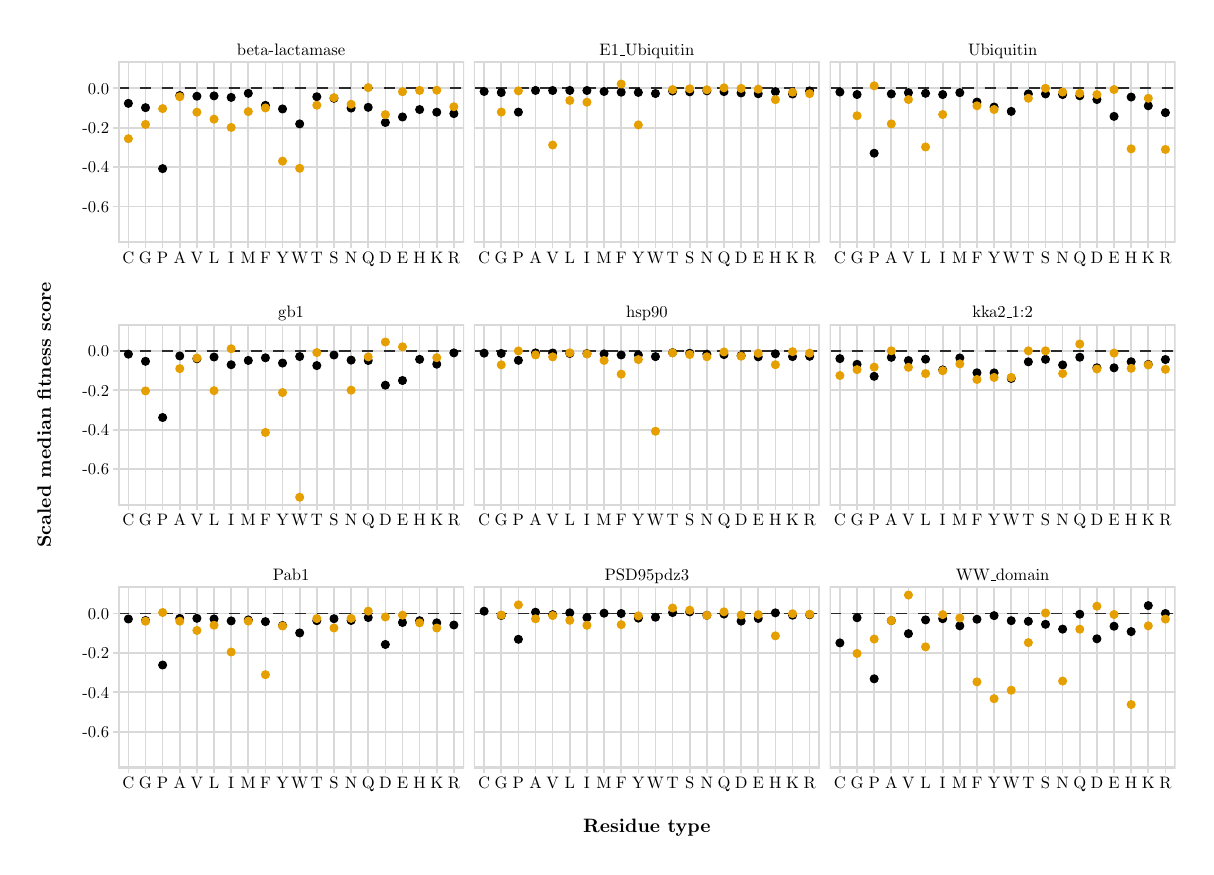
\begin{tikzpicture}[x=1pt,y=1pt]
\definecolor{fillColor}{RGB}{255,255,255}
\path[use as bounding box,fill=fillColor,fill opacity=0.00] (0,0) rectangle (418.34,295.82);
\begin{scope}
\path[clip] ( 32.67,218.05) rectangle (157.73,283.52);
\definecolor{drawColor}{gray}{0.85}

\path[draw=drawColor,line width= 0.6pt,line join=round] ( 32.67,231.15) --
	(157.73,231.15);

\path[draw=drawColor,line width= 0.6pt,line join=round] ( 32.67,245.40) --
	(157.73,245.40);

\path[draw=drawColor,line width= 0.6pt,line join=round] ( 32.67,259.66) --
	(157.73,259.66);

\path[draw=drawColor,line width= 0.6pt,line join=round] ( 32.67,273.91) --
	(157.73,273.91);

\path[draw=drawColor,line width= 0.6pt,line join=round] ( 36.39,218.05) --
	( 36.39,283.52);

\path[draw=drawColor,line width= 0.6pt,line join=round] ( 42.58,218.05) --
	( 42.58,283.52);

\path[draw=drawColor,line width= 0.6pt,line join=round] ( 48.77,218.05) --
	( 48.77,283.52);

\path[draw=drawColor,line width= 0.6pt,line join=round] ( 54.96,218.05) --
	( 54.96,283.52);

\path[draw=drawColor,line width= 0.6pt,line join=round] ( 61.15,218.05) --
	( 61.15,283.52);

\path[draw=drawColor,line width= 0.6pt,line join=round] ( 67.34,218.05) --
	( 67.34,283.52);

\path[draw=drawColor,line width= 0.6pt,line join=round] ( 73.53,218.05) --
	( 73.53,283.52);

\path[draw=drawColor,line width= 0.6pt,line join=round] ( 79.72,218.05) --
	( 79.72,283.52);

\path[draw=drawColor,line width= 0.6pt,line join=round] ( 85.91,218.05) --
	( 85.91,283.52);

\path[draw=drawColor,line width= 0.6pt,line join=round] ( 92.10,218.05) --
	( 92.10,283.52);

\path[draw=drawColor,line width= 0.6pt,line join=round] ( 98.29,218.05) --
	( 98.29,283.52);

\path[draw=drawColor,line width= 0.6pt,line join=round] (104.48,218.05) --
	(104.48,283.52);

\path[draw=drawColor,line width= 0.6pt,line join=round] (110.68,218.05) --
	(110.68,283.52);

\path[draw=drawColor,line width= 0.6pt,line join=round] (116.87,218.05) --
	(116.87,283.52);

\path[draw=drawColor,line width= 0.6pt,line join=round] (123.06,218.05) --
	(123.06,283.52);

\path[draw=drawColor,line width= 0.6pt,line join=round] (129.25,218.05) --
	(129.25,283.52);

\path[draw=drawColor,line width= 0.6pt,line join=round] (135.44,218.05) --
	(135.44,283.52);

\path[draw=drawColor,line width= 0.6pt,line join=round] (141.63,218.05) --
	(141.63,283.52);

\path[draw=drawColor,line width= 0.6pt,line join=round] (147.82,218.05) --
	(147.82,283.52);

\path[draw=drawColor,line width= 0.6pt,line join=round] (154.01,218.05) --
	(154.01,283.52);
\definecolor{drawColor}{RGB}{0,0,0}

\path[draw=drawColor,draw opacity=0.80,line width= 0.6pt,dash pattern=on 4pt off 4pt ,line join=round] ( 32.67,273.91) -- (157.73,273.91);
\definecolor{drawColor}{RGB}{0,0,0}
\definecolor{fillColor}{RGB}{0,0,0}

\path[draw=drawColor,line width= 0.4pt,line join=round,line cap=round,fill=fillColor] ( 48.77,244.88) circle (  1.43);

\path[draw=drawColor,line width= 0.4pt,line join=round,line cap=round,fill=fillColor] (123.06,267.04) circle (  1.43);

\path[draw=drawColor,line width= 0.4pt,line join=round,line cap=round,fill=fillColor] (129.25,261.55) circle (  1.43);

\path[draw=drawColor,line width= 0.4pt,line join=round,line cap=round,fill=fillColor] (147.82,265.27) circle (  1.43);

\path[draw=drawColor,line width= 0.4pt,line join=round,line cap=round,fill=fillColor] (116.87,266.76) circle (  1.43);

\path[draw=drawColor,line width= 0.4pt,line join=round,line cap=round,fill=fillColor] (154.01,264.76) circle (  1.43);

\path[draw=drawColor,line width= 0.4pt,line join=round,line cap=round,fill=fillColor] (135.44,263.55) circle (  1.43);

\path[draw=drawColor,line width= 0.4pt,line join=round,line cap=round,fill=fillColor] (141.63,266.23) circle (  1.43);

\path[draw=drawColor,line width= 0.4pt,line join=round,line cap=round,fill=fillColor] (110.68,270.30) circle (  1.43);

\path[draw=drawColor,line width= 0.4pt,line join=round,line cap=round,fill=fillColor] (104.48,270.86) circle (  1.43);

\path[draw=drawColor,line width= 0.4pt,line join=round,line cap=round,fill=fillColor] ( 42.58,266.91) circle (  1.43);

\path[draw=drawColor,line width= 0.4pt,line join=round,line cap=round,fill=fillColor] ( 36.39,268.46) circle (  1.43);

\path[draw=drawColor,line width= 0.4pt,line join=round,line cap=round,fill=fillColor] ( 54.96,271.30) circle (  1.43);

\path[draw=drawColor,line width= 0.4pt,line join=round,line cap=round,fill=fillColor] ( 79.72,272.10) circle (  1.43);

\path[draw=drawColor,line width= 0.4pt,line join=round,line cap=round,fill=fillColor] ( 61.15,271.05) circle (  1.43);

\path[draw=drawColor,line width= 0.4pt,line join=round,line cap=round,fill=fillColor] ( 92.10,266.45) circle (  1.43);

\path[draw=drawColor,line width= 0.4pt,line join=round,line cap=round,fill=fillColor] ( 85.91,267.75) circle (  1.43);

\path[draw=drawColor,line width= 0.4pt,line join=round,line cap=round,fill=fillColor] ( 67.34,271.17) circle (  1.43);

\path[draw=drawColor,line width= 0.4pt,line join=round,line cap=round,fill=fillColor] ( 73.53,270.62) circle (  1.43);

\path[draw=drawColor,line width= 0.4pt,line join=round,line cap=round,fill=fillColor] ( 98.29,261.04) circle (  1.43);
\definecolor{drawColor}{RGB}{230,159,0}
\definecolor{fillColor}{RGB}{230,159,0}

\path[draw=drawColor,line width= 0.4pt,line join=round,line cap=round,fill=fillColor] ( 48.77,266.57) circle (  1.43);

\path[draw=drawColor,line width= 0.4pt,line join=round,line cap=round,fill=fillColor] (129.25,264.40) circle (  1.43);

\path[draw=drawColor,line width= 0.4pt,line join=round,line cap=round,fill=fillColor] ( 54.96,270.86) circle (  1.43);

\path[draw=drawColor,line width= 0.4pt,line join=round,line cap=round,fill=fillColor] ( 36.39,255.70) circle (  1.43);

\path[draw=drawColor,line width= 0.4pt,line join=round,line cap=round,fill=fillColor] (116.87,268.15) circle (  1.43);

\path[draw=drawColor,line width= 0.4pt,line join=round,line cap=round,fill=fillColor] ( 67.34,262.76) circle (  1.43);

\path[draw=drawColor,line width= 0.4pt,line join=round,line cap=round,fill=fillColor] ( 85.91,266.81) circle (  1.43);

\path[draw=drawColor,line width= 0.4pt,line join=round,line cap=round,fill=fillColor] (135.44,272.68) circle (  1.43);

\path[draw=drawColor,line width= 0.4pt,line join=round,line cap=round,fill=fillColor] (141.63,273.14) circle (  1.43);

\path[draw=drawColor,line width= 0.4pt,line join=round,line cap=round,fill=fillColor] (104.48,267.79) circle (  1.43);

\path[draw=drawColor,line width= 0.4pt,line join=round,line cap=round,fill=fillColor] ( 73.53,259.76) circle (  1.43);

\path[draw=drawColor,line width= 0.4pt,line join=round,line cap=round,fill=fillColor] (154.01,267.24) circle (  1.43);

\path[draw=drawColor,line width= 0.4pt,line join=round,line cap=round,fill=fillColor] ( 61.15,265.28) circle (  1.43);

\path[draw=drawColor,line width= 0.4pt,line join=round,line cap=round,fill=fillColor] ( 92.10,247.60) circle (  1.43);

\path[draw=drawColor,line width= 0.4pt,line join=round,line cap=round,fill=fillColor] (123.06,274.16) circle (  1.43);

\path[draw=drawColor,line width= 0.4pt,line join=round,line cap=round,fill=fillColor] ( 42.58,260.85) circle (  1.43);

\path[draw=drawColor,line width= 0.4pt,line join=round,line cap=round,fill=fillColor] (147.82,273.22) circle (  1.43);

\path[draw=drawColor,line width= 0.4pt,line join=round,line cap=round,fill=fillColor] (110.68,270.52) circle (  1.43);

\path[draw=drawColor,line width= 0.4pt,line join=round,line cap=round,fill=fillColor] ( 79.72,265.50) circle (  1.43);

\path[draw=drawColor,line width= 0.4pt,line join=round,line cap=round,fill=fillColor] ( 98.29,245.00) circle (  1.43);
\definecolor{drawColor}{gray}{0.85}

\path[draw=drawColor,line width= 1.1pt,line join=round,line cap=round] ( 32.67,218.05) rectangle (157.73,283.52);
\end{scope}
\begin{scope}
\path[clip] ( 32.67,123.17) rectangle (157.73,188.65);
\definecolor{drawColor}{gray}{0.85}

\path[draw=drawColor,line width= 0.6pt,line join=round] ( 32.67,136.28) --
	(157.73,136.28);

\path[draw=drawColor,line width= 0.6pt,line join=round] ( 32.67,150.53) --
	(157.73,150.53);

\path[draw=drawColor,line width= 0.6pt,line join=round] ( 32.67,164.78) --
	(157.73,164.78);

\path[draw=drawColor,line width= 0.6pt,line join=round] ( 32.67,179.04) --
	(157.73,179.04);

\path[draw=drawColor,line width= 0.6pt,line join=round] ( 36.39,123.17) --
	( 36.39,188.65);

\path[draw=drawColor,line width= 0.6pt,line join=round] ( 42.58,123.17) --
	( 42.58,188.65);

\path[draw=drawColor,line width= 0.6pt,line join=round] ( 48.77,123.17) --
	( 48.77,188.65);

\path[draw=drawColor,line width= 0.6pt,line join=round] ( 54.96,123.17) --
	( 54.96,188.65);

\path[draw=drawColor,line width= 0.6pt,line join=round] ( 61.15,123.17) --
	( 61.15,188.65);

\path[draw=drawColor,line width= 0.6pt,line join=round] ( 67.34,123.17) --
	( 67.34,188.65);

\path[draw=drawColor,line width= 0.6pt,line join=round] ( 73.53,123.17) --
	( 73.53,188.65);

\path[draw=drawColor,line width= 0.6pt,line join=round] ( 79.72,123.17) --
	( 79.72,188.65);

\path[draw=drawColor,line width= 0.6pt,line join=round] ( 85.91,123.17) --
	( 85.91,188.65);

\path[draw=drawColor,line width= 0.6pt,line join=round] ( 92.10,123.17) --
	( 92.10,188.65);

\path[draw=drawColor,line width= 0.6pt,line join=round] ( 98.29,123.17) --
	( 98.29,188.65);

\path[draw=drawColor,line width= 0.6pt,line join=round] (104.48,123.17) --
	(104.48,188.65);

\path[draw=drawColor,line width= 0.6pt,line join=round] (110.68,123.17) --
	(110.68,188.65);

\path[draw=drawColor,line width= 0.6pt,line join=round] (116.87,123.17) --
	(116.87,188.65);

\path[draw=drawColor,line width= 0.6pt,line join=round] (123.06,123.17) --
	(123.06,188.65);

\path[draw=drawColor,line width= 0.6pt,line join=round] (129.25,123.17) --
	(129.25,188.65);

\path[draw=drawColor,line width= 0.6pt,line join=round] (135.44,123.17) --
	(135.44,188.65);

\path[draw=drawColor,line width= 0.6pt,line join=round] (141.63,123.17) --
	(141.63,188.65);

\path[draw=drawColor,line width= 0.6pt,line join=round] (147.82,123.17) --
	(147.82,188.65);

\path[draw=drawColor,line width= 0.6pt,line join=round] (154.01,123.17) --
	(154.01,188.65);
\definecolor{drawColor}{RGB}{0,0,0}

\path[draw=drawColor,draw opacity=0.80,line width= 0.6pt,dash pattern=on 4pt off 4pt ,line join=round] ( 32.67,179.04) -- (157.73,179.04);
\definecolor{drawColor}{RGB}{0,0,0}
\definecolor{fillColor}{RGB}{0,0,0}

\path[draw=drawColor,line width= 0.4pt,line join=round,line cap=round,fill=fillColor] ( 92.10,174.63) circle (  1.43);

\path[draw=drawColor,line width= 0.4pt,line join=round,line cap=round,fill=fillColor] ( 98.29,176.98) circle (  1.43);

\path[draw=drawColor,line width= 0.4pt,line join=round,line cap=round,fill=fillColor] (141.63,175.97) circle (  1.43);

\path[draw=drawColor,line width= 0.4pt,line join=round,line cap=round,fill=fillColor] ( 85.91,176.52) circle (  1.43);

\path[draw=drawColor,line width= 0.4pt,line join=round,line cap=round,fill=fillColor] (135.44,168.32) circle (  1.43);

\path[draw=drawColor,line width= 0.4pt,line join=round,line cap=round,fill=fillColor] ( 48.77,154.95) circle (  1.43);

\path[draw=drawColor,line width= 0.4pt,line join=round,line cap=round,fill=fillColor] (123.06,175.55) circle (  1.43);

\path[draw=drawColor,line width= 0.4pt,line join=round,line cap=round,fill=fillColor] ( 42.58,175.26) circle (  1.43);

\path[draw=drawColor,line width= 0.4pt,line join=round,line cap=round,fill=fillColor] (116.87,175.69) circle (  1.43);

\path[draw=drawColor,line width= 0.4pt,line join=round,line cap=round,fill=fillColor] (104.48,173.71) circle (  1.43);

\path[draw=drawColor,line width= 0.4pt,line join=round,line cap=round,fill=fillColor] ( 79.72,175.57) circle (  1.43);

\path[draw=drawColor,line width= 0.4pt,line join=round,line cap=round,fill=fillColor] (110.68,177.53) circle (  1.43);

\path[draw=drawColor,line width= 0.4pt,line join=round,line cap=round,fill=fillColor] ( 36.39,177.85) circle (  1.43);

\path[draw=drawColor,line width= 0.4pt,line join=round,line cap=round,fill=fillColor] ( 61.15,176.18) circle (  1.43);

\path[draw=drawColor,line width= 0.4pt,line join=round,line cap=round,fill=fillColor] ( 73.53,174.02) circle (  1.43);

\path[draw=drawColor,line width= 0.4pt,line join=round,line cap=round,fill=fillColor] ( 67.34,176.81) circle (  1.43);

\path[draw=drawColor,line width= 0.4pt,line join=round,line cap=round,fill=fillColor] (129.25,166.63) circle (  1.43);

\path[draw=drawColor,line width= 0.4pt,line join=round,line cap=round,fill=fillColor] (154.01,178.30) circle (  1.43);

\path[draw=drawColor,line width= 0.4pt,line join=round,line cap=round,fill=fillColor] (147.82,174.23) circle (  1.43);

\path[draw=drawColor,line width= 0.4pt,line join=round,line cap=round,fill=fillColor] ( 54.96,177.20) circle (  1.43);
\definecolor{drawColor}{RGB}{230,159,0}
\definecolor{fillColor}{RGB}{230,159,0}

\path[draw=drawColor,line width= 0.4pt,line join=round,line cap=round,fill=fillColor] ( 54.96,172.61) circle (  1.43);

\path[draw=drawColor,line width= 0.4pt,line join=round,line cap=round,fill=fillColor] (129.25,182.23) circle (  1.43);

\path[draw=drawColor,line width= 0.4pt,line join=round,line cap=round,fill=fillColor] ( 61.15,176.46) circle (  1.43);

\path[draw=drawColor,line width= 0.4pt,line join=round,line cap=round,fill=fillColor] (104.48,178.42) circle (  1.43);

\path[draw=drawColor,line width= 0.4pt,line join=round,line cap=round,fill=fillColor] (135.44,180.50) circle (  1.43);

\path[draw=drawColor,line width= 0.4pt,line join=round,line cap=round,fill=fillColor] (147.82,176.56) circle (  1.43);

\path[draw=drawColor,line width= 0.4pt,line join=round,line cap=round,fill=fillColor] ( 92.10,163.97) circle (  1.43);

\path[draw=drawColor,line width= 0.4pt,line join=round,line cap=round,fill=fillColor] ( 67.34,164.65) circle (  1.43);

\path[draw=drawColor,line width= 0.4pt,line join=round,line cap=round,fill=fillColor] (123.06,176.87) circle (  1.43);

\path[draw=drawColor,line width= 0.4pt,line join=round,line cap=round,fill=fillColor] (116.87,164.83) circle (  1.43);

\path[draw=drawColor,line width= 0.4pt,line join=round,line cap=round,fill=fillColor] ( 73.53,179.80) circle (  1.43);

\path[draw=drawColor,line width= 0.4pt,line join=round,line cap=round,fill=fillColor] ( 42.58,164.56) circle (  1.43);

\path[draw=drawColor,line width= 0.4pt,line join=round,line cap=round,fill=fillColor] ( 85.91,149.55) circle (  1.43);

\path[draw=drawColor,line width= 0.4pt,line join=round,line cap=round,fill=fillColor] ( 98.29,126.15) circle (  1.43);
\definecolor{drawColor}{gray}{0.85}

\path[draw=drawColor,line width= 1.1pt,line join=round,line cap=round] ( 32.67,123.17) rectangle (157.73,188.65);
\end{scope}
\begin{scope}
\path[clip] ( 32.67, 28.30) rectangle (157.73, 93.78);
\definecolor{drawColor}{gray}{0.85}

\path[draw=drawColor,line width= 0.6pt,line join=round] ( 32.67, 41.40) --
	(157.73, 41.40);

\path[draw=drawColor,line width= 0.6pt,line join=round] ( 32.67, 55.66) --
	(157.73, 55.66);

\path[draw=drawColor,line width= 0.6pt,line join=round] ( 32.67, 69.91) --
	(157.73, 69.91);

\path[draw=drawColor,line width= 0.6pt,line join=round] ( 32.67, 84.17) --
	(157.73, 84.17);

\path[draw=drawColor,line width= 0.6pt,line join=round] ( 36.39, 28.30) --
	( 36.39, 93.78);

\path[draw=drawColor,line width= 0.6pt,line join=round] ( 42.58, 28.30) --
	( 42.58, 93.78);

\path[draw=drawColor,line width= 0.6pt,line join=round] ( 48.77, 28.30) --
	( 48.77, 93.78);

\path[draw=drawColor,line width= 0.6pt,line join=round] ( 54.96, 28.30) --
	( 54.96, 93.78);

\path[draw=drawColor,line width= 0.6pt,line join=round] ( 61.15, 28.30) --
	( 61.15, 93.78);

\path[draw=drawColor,line width= 0.6pt,line join=round] ( 67.34, 28.30) --
	( 67.34, 93.78);

\path[draw=drawColor,line width= 0.6pt,line join=round] ( 73.53, 28.30) --
	( 73.53, 93.78);

\path[draw=drawColor,line width= 0.6pt,line join=round] ( 79.72, 28.30) --
	( 79.72, 93.78);

\path[draw=drawColor,line width= 0.6pt,line join=round] ( 85.91, 28.30) --
	( 85.91, 93.78);

\path[draw=drawColor,line width= 0.6pt,line join=round] ( 92.10, 28.30) --
	( 92.10, 93.78);

\path[draw=drawColor,line width= 0.6pt,line join=round] ( 98.29, 28.30) --
	( 98.29, 93.78);

\path[draw=drawColor,line width= 0.6pt,line join=round] (104.48, 28.30) --
	(104.48, 93.78);

\path[draw=drawColor,line width= 0.6pt,line join=round] (110.68, 28.30) --
	(110.68, 93.78);

\path[draw=drawColor,line width= 0.6pt,line join=round] (116.87, 28.30) --
	(116.87, 93.78);

\path[draw=drawColor,line width= 0.6pt,line join=round] (123.06, 28.30) --
	(123.06, 93.78);

\path[draw=drawColor,line width= 0.6pt,line join=round] (129.25, 28.30) --
	(129.25, 93.78);

\path[draw=drawColor,line width= 0.6pt,line join=round] (135.44, 28.30) --
	(135.44, 93.78);

\path[draw=drawColor,line width= 0.6pt,line join=round] (141.63, 28.30) --
	(141.63, 93.78);

\path[draw=drawColor,line width= 0.6pt,line join=round] (147.82, 28.30) --
	(147.82, 93.78);

\path[draw=drawColor,line width= 0.6pt,line join=round] (154.01, 28.30) --
	(154.01, 93.78);
\definecolor{drawColor}{RGB}{0,0,0}

\path[draw=drawColor,draw opacity=0.80,line width= 0.6pt,dash pattern=on 4pt off 4pt ,line join=round] ( 32.67, 84.17) -- (157.73, 84.17);
\definecolor{drawColor}{RGB}{0,0,0}
\definecolor{fillColor}{RGB}{0,0,0}

\path[draw=drawColor,line width= 0.4pt,line join=round,line cap=round,fill=fillColor] ( 36.39, 82.14) circle (  1.43);

\path[draw=drawColor,line width= 0.4pt,line join=round,line cap=round,fill=fillColor] (116.87, 81.60) circle (  1.43);

\path[draw=drawColor,line width= 0.4pt,line join=round,line cap=round,fill=fillColor] (110.68, 82.25) circle (  1.43);

\path[draw=drawColor,line width= 0.4pt,line join=round,line cap=round,fill=fillColor] (154.01, 79.97) circle (  1.43);

\path[draw=drawColor,line width= 0.4pt,line join=round,line cap=round,fill=fillColor] (141.63, 81.53) circle (  1.43);

\path[draw=drawColor,line width= 0.4pt,line join=round,line cap=round,fill=fillColor] ( 54.96, 82.37) circle (  1.43);

\path[draw=drawColor,line width= 0.4pt,line join=round,line cap=round,fill=fillColor] (135.44, 80.88) circle (  1.43);

\path[draw=drawColor,line width= 0.4pt,line join=round,line cap=round,fill=fillColor] (104.48, 81.53) circle (  1.43);

\path[draw=drawColor,line width= 0.4pt,line join=round,line cap=round,fill=fillColor] ( 67.34, 82.17) circle (  1.43);

\path[draw=drawColor,line width= 0.4pt,line join=round,line cap=round,fill=fillColor] (147.82, 80.76) circle (  1.43);

\path[draw=drawColor,line width= 0.4pt,line join=round,line cap=round,fill=fillColor] (129.25, 72.94) circle (  1.43);

\path[draw=drawColor,line width= 0.4pt,line join=round,line cap=round,fill=fillColor] ( 42.58, 81.60) circle (  1.43);

\path[draw=drawColor,line width= 0.4pt,line join=round,line cap=round,fill=fillColor] ( 92.10, 79.79) circle (  1.43);

\path[draw=drawColor,line width= 0.4pt,line join=round,line cap=round,fill=fillColor] ( 61.15, 82.39) circle (  1.43);

\path[draw=drawColor,line width= 0.4pt,line join=round,line cap=round,fill=fillColor] ( 73.53, 81.45) circle (  1.43);

\path[draw=drawColor,line width= 0.4pt,line join=round,line cap=round,fill=fillColor] ( 48.77, 65.51) circle (  1.43);

\path[draw=drawColor,line width= 0.4pt,line join=round,line cap=round,fill=fillColor] ( 85.91, 81.19) circle (  1.43);

\path[draw=drawColor,line width= 0.4pt,line join=round,line cap=round,fill=fillColor] ( 79.72, 81.81) circle (  1.43);

\path[draw=drawColor,line width= 0.4pt,line join=round,line cap=round,fill=fillColor] (123.06, 82.68) circle (  1.43);

\path[draw=drawColor,line width= 0.4pt,line join=round,line cap=round,fill=fillColor] ( 98.29, 77.11) circle (  1.43);
\definecolor{drawColor}{RGB}{230,159,0}
\definecolor{fillColor}{RGB}{230,159,0}

\path[draw=drawColor,line width= 0.4pt,line join=round,line cap=round,fill=fillColor] (123.06, 84.99) circle (  1.43);

\path[draw=drawColor,line width= 0.4pt,line join=round,line cap=round,fill=fillColor] ( 54.96, 81.36) circle (  1.43);

\path[draw=drawColor,line width= 0.4pt,line join=round,line cap=round,fill=fillColor] (116.87, 82.37) circle (  1.43);

\path[draw=drawColor,line width= 0.4pt,line join=round,line cap=round,fill=fillColor] ( 48.77, 84.49) circle (  1.43);

\path[draw=drawColor,line width= 0.4pt,line join=round,line cap=round,fill=fillColor] ( 42.58, 81.34) circle (  1.43);

\path[draw=drawColor,line width= 0.4pt,line join=round,line cap=round,fill=fillColor] (104.48, 82.30) circle (  1.43);

\path[draw=drawColor,line width= 0.4pt,line join=round,line cap=round,fill=fillColor] (135.44, 83.53) circle (  1.43);

\path[draw=drawColor,line width= 0.4pt,line join=round,line cap=round,fill=fillColor] (129.25, 82.88) circle (  1.43);

\path[draw=drawColor,line width= 0.4pt,line join=round,line cap=round,fill=fillColor] ( 61.15, 78.01) circle (  1.43);

\path[draw=drawColor,line width= 0.4pt,line join=round,line cap=round,fill=fillColor] ( 67.34, 79.89) circle (  1.43);

\path[draw=drawColor,line width= 0.4pt,line join=round,line cap=round,fill=fillColor] (110.68, 78.90) circle (  1.43);

\path[draw=drawColor,line width= 0.4pt,line join=round,line cap=round,fill=fillColor] (147.82, 78.89) circle (  1.43);

\path[draw=drawColor,line width= 0.4pt,line join=round,line cap=round,fill=fillColor] ( 73.53, 70.21) circle (  1.43);

\path[draw=drawColor,line width= 0.4pt,line join=round,line cap=round,fill=fillColor] (141.63, 80.76) circle (  1.43);

\path[draw=drawColor,line width= 0.4pt,line join=round,line cap=round,fill=fillColor] ( 79.72, 81.39) circle (  1.43);

\path[draw=drawColor,line width= 0.4pt,line join=round,line cap=round,fill=fillColor] ( 85.91, 62.03) circle (  1.43);

\path[draw=drawColor,line width= 0.4pt,line join=round,line cap=round,fill=fillColor] ( 92.10, 79.62) circle (  1.43);
\definecolor{drawColor}{gray}{0.85}

\path[draw=drawColor,line width= 1.1pt,line join=round,line cap=round] ( 32.67, 28.30) rectangle (157.73, 93.78);
\end{scope}
\begin{scope}
\path[clip] (161.23,218.05) rectangle (286.28,283.52);
\definecolor{drawColor}{gray}{0.85}

\path[draw=drawColor,line width= 0.6pt,line join=round] (161.23,231.15) --
	(286.28,231.15);

\path[draw=drawColor,line width= 0.6pt,line join=round] (161.23,245.40) --
	(286.28,245.40);

\path[draw=drawColor,line width= 0.6pt,line join=round] (161.23,259.66) --
	(286.28,259.66);

\path[draw=drawColor,line width= 0.6pt,line join=round] (161.23,273.91) --
	(286.28,273.91);

\path[draw=drawColor,line width= 0.6pt,line join=round] (164.94,218.05) --
	(164.94,283.52);

\path[draw=drawColor,line width= 0.6pt,line join=round] (171.13,218.05) --
	(171.13,283.52);

\path[draw=drawColor,line width= 0.6pt,line join=round] (177.32,218.05) --
	(177.32,283.52);

\path[draw=drawColor,line width= 0.6pt,line join=round] (183.51,218.05) --
	(183.51,283.52);

\path[draw=drawColor,line width= 0.6pt,line join=round] (189.70,218.05) --
	(189.70,283.52);

\path[draw=drawColor,line width= 0.6pt,line join=round] (195.89,218.05) --
	(195.89,283.52);

\path[draw=drawColor,line width= 0.6pt,line join=round] (202.09,218.05) --
	(202.09,283.52);

\path[draw=drawColor,line width= 0.6pt,line join=round] (208.28,218.05) --
	(208.28,283.52);

\path[draw=drawColor,line width= 0.6pt,line join=round] (214.47,218.05) --
	(214.47,283.52);

\path[draw=drawColor,line width= 0.6pt,line join=round] (220.66,218.05) --
	(220.66,283.52);

\path[draw=drawColor,line width= 0.6pt,line join=round] (226.85,218.05) --
	(226.85,283.52);

\path[draw=drawColor,line width= 0.6pt,line join=round] (233.04,218.05) --
	(233.04,283.52);

\path[draw=drawColor,line width= 0.6pt,line join=round] (239.23,218.05) --
	(239.23,283.52);

\path[draw=drawColor,line width= 0.6pt,line join=round] (245.42,218.05) --
	(245.42,283.52);

\path[draw=drawColor,line width= 0.6pt,line join=round] (251.61,218.05) --
	(251.61,283.52);

\path[draw=drawColor,line width= 0.6pt,line join=round] (257.80,218.05) --
	(257.80,283.52);

\path[draw=drawColor,line width= 0.6pt,line join=round] (263.99,218.05) --
	(263.99,283.52);

\path[draw=drawColor,line width= 0.6pt,line join=round] (270.18,218.05) --
	(270.18,283.52);

\path[draw=drawColor,line width= 0.6pt,line join=round] (276.38,218.05) --
	(276.38,283.52);

\path[draw=drawColor,line width= 0.6pt,line join=round] (282.57,218.05) --
	(282.57,283.52);
\definecolor{drawColor}{RGB}{0,0,0}

\path[draw=drawColor,draw opacity=0.80,line width= 0.6pt,dash pattern=on 4pt off 4pt ,line join=round] (161.23,273.91) -- (286.28,273.91);
\definecolor{drawColor}{RGB}{0,0,0}
\definecolor{fillColor}{RGB}{0,0,0}

\path[draw=drawColor,line width= 0.4pt,line join=round,line cap=round,fill=fillColor] (164.94,272.77) circle (  1.43);

\path[draw=drawColor,line width= 0.4pt,line join=round,line cap=round,fill=fillColor] (220.66,272.42) circle (  1.43);

\path[draw=drawColor,line width= 0.4pt,line join=round,line cap=round,fill=fillColor] (214.47,272.51) circle (  1.43);

\path[draw=drawColor,line width= 0.4pt,line join=round,line cap=round,fill=fillColor] (171.13,272.38) circle (  1.43);

\path[draw=drawColor,line width= 0.4pt,line join=round,line cap=round,fill=fillColor] (239.23,272.63) circle (  1.43);

\path[draw=drawColor,line width= 0.4pt,line join=round,line cap=round,fill=fillColor] (233.04,272.91) circle (  1.43);

\path[draw=drawColor,line width= 0.4pt,line join=round,line cap=round,fill=fillColor] (202.09,273.11) circle (  1.43);

\path[draw=drawColor,line width= 0.4pt,line join=round,line cap=round,fill=fillColor] (195.89,273.14) circle (  1.43);

\path[draw=drawColor,line width= 0.4pt,line join=round,line cap=round,fill=fillColor] (282.57,272.96) circle (  1.43);

\path[draw=drawColor,line width= 0.4pt,line join=round,line cap=round,fill=fillColor] (177.32,265.30) circle (  1.43);

\path[draw=drawColor,line width= 0.4pt,line join=round,line cap=round,fill=fillColor] (257.80,272.23) circle (  1.43);

\path[draw=drawColor,line width= 0.4pt,line join=round,line cap=round,fill=fillColor] (270.18,272.72) circle (  1.43);

\path[draw=drawColor,line width= 0.4pt,line join=round,line cap=round,fill=fillColor] (183.51,273.14) circle (  1.43);

\path[draw=drawColor,line width= 0.4pt,line join=round,line cap=round,fill=fillColor] (208.28,272.77) circle (  1.43);

\path[draw=drawColor,line width= 0.4pt,line join=round,line cap=round,fill=fillColor] (276.38,271.85) circle (  1.43);

\path[draw=drawColor,line width= 0.4pt,line join=round,line cap=round,fill=fillColor] (189.70,273.11) circle (  1.43);

\path[draw=drawColor,line width= 0.4pt,line join=round,line cap=round,fill=fillColor] (226.85,272.02) circle (  1.43);

\path[draw=drawColor,line width= 0.4pt,line join=round,line cap=round,fill=fillColor] (245.42,273.00) circle (  1.43);

\path[draw=drawColor,line width= 0.4pt,line join=round,line cap=round,fill=fillColor] (263.99,271.95) circle (  1.43);

\path[draw=drawColor,line width= 0.4pt,line join=round,line cap=round,fill=fillColor] (251.61,272.72) circle (  1.43);
\definecolor{drawColor}{RGB}{230,159,0}
\definecolor{fillColor}{RGB}{230,159,0}

\path[draw=drawColor,line width= 0.4pt,line join=round,line cap=round,fill=fillColor] (251.61,274.08) circle (  1.43);

\path[draw=drawColor,line width= 0.4pt,line join=round,line cap=round,fill=fillColor] (257.80,273.88) circle (  1.43);

\path[draw=drawColor,line width= 0.4pt,line join=round,line cap=round,fill=fillColor] (214.47,275.45) circle (  1.43);

\path[draw=drawColor,line width= 0.4pt,line join=round,line cap=round,fill=fillColor] (233.04,273.44) circle (  1.43);

\path[draw=drawColor,line width= 0.4pt,line join=round,line cap=round,fill=fillColor] (263.99,273.61) circle (  1.43);

\path[draw=drawColor,line width= 0.4pt,line join=round,line cap=round,fill=fillColor] (189.70,253.41) circle (  1.43);

\path[draw=drawColor,line width= 0.4pt,line join=round,line cap=round,fill=fillColor] (195.89,269.51) circle (  1.43);

\path[draw=drawColor,line width= 0.4pt,line join=round,line cap=round,fill=fillColor] (239.23,273.73) circle (  1.43);

\path[draw=drawColor,line width= 0.4pt,line join=round,line cap=round,fill=fillColor] (202.09,268.89) circle (  1.43);

\path[draw=drawColor,line width= 0.4pt,line join=round,line cap=round,fill=fillColor] (220.66,260.68) circle (  1.43);

\path[draw=drawColor,line width= 0.4pt,line join=round,line cap=round,fill=fillColor] (276.38,272.49) circle (  1.43);

\path[draw=drawColor,line width= 0.4pt,line join=round,line cap=round,fill=fillColor] (245.42,273.39) circle (  1.43);

\path[draw=drawColor,line width= 0.4pt,line join=round,line cap=round,fill=fillColor] (270.18,269.81) circle (  1.43);

\path[draw=drawColor,line width= 0.4pt,line join=round,line cap=round,fill=fillColor] (177.32,272.98) circle (  1.43);

\path[draw=drawColor,line width= 0.4pt,line join=round,line cap=round,fill=fillColor] (282.57,271.98) circle (  1.43);

\path[draw=drawColor,line width= 0.4pt,line join=round,line cap=round,fill=fillColor] (171.13,265.33) circle (  1.43);
\definecolor{drawColor}{gray}{0.85}

\path[draw=drawColor,line width= 1.1pt,line join=round,line cap=round] (161.23,218.05) rectangle (286.28,283.52);
\end{scope}
\begin{scope}
\path[clip] (161.23,123.17) rectangle (286.28,188.65);
\definecolor{drawColor}{gray}{0.85}

\path[draw=drawColor,line width= 0.6pt,line join=round] (161.23,136.28) --
	(286.28,136.28);

\path[draw=drawColor,line width= 0.6pt,line join=round] (161.23,150.53) --
	(286.28,150.53);

\path[draw=drawColor,line width= 0.6pt,line join=round] (161.23,164.78) --
	(286.28,164.78);

\path[draw=drawColor,line width= 0.6pt,line join=round] (161.23,179.04) --
	(286.28,179.04);

\path[draw=drawColor,line width= 0.6pt,line join=round] (164.94,123.17) --
	(164.94,188.65);

\path[draw=drawColor,line width= 0.6pt,line join=round] (171.13,123.17) --
	(171.13,188.65);

\path[draw=drawColor,line width= 0.6pt,line join=round] (177.32,123.17) --
	(177.32,188.65);

\path[draw=drawColor,line width= 0.6pt,line join=round] (183.51,123.17) --
	(183.51,188.65);

\path[draw=drawColor,line width= 0.6pt,line join=round] (189.70,123.17) --
	(189.70,188.65);

\path[draw=drawColor,line width= 0.6pt,line join=round] (195.89,123.17) --
	(195.89,188.65);

\path[draw=drawColor,line width= 0.6pt,line join=round] (202.09,123.17) --
	(202.09,188.65);

\path[draw=drawColor,line width= 0.6pt,line join=round] (208.28,123.17) --
	(208.28,188.65);

\path[draw=drawColor,line width= 0.6pt,line join=round] (214.47,123.17) --
	(214.47,188.65);

\path[draw=drawColor,line width= 0.6pt,line join=round] (220.66,123.17) --
	(220.66,188.65);

\path[draw=drawColor,line width= 0.6pt,line join=round] (226.85,123.17) --
	(226.85,188.65);

\path[draw=drawColor,line width= 0.6pt,line join=round] (233.04,123.17) --
	(233.04,188.65);

\path[draw=drawColor,line width= 0.6pt,line join=round] (239.23,123.17) --
	(239.23,188.65);

\path[draw=drawColor,line width= 0.6pt,line join=round] (245.42,123.17) --
	(245.42,188.65);

\path[draw=drawColor,line width= 0.6pt,line join=round] (251.61,123.17) --
	(251.61,188.65);

\path[draw=drawColor,line width= 0.6pt,line join=round] (257.80,123.17) --
	(257.80,188.65);

\path[draw=drawColor,line width= 0.6pt,line join=round] (263.99,123.17) --
	(263.99,188.65);

\path[draw=drawColor,line width= 0.6pt,line join=round] (270.18,123.17) --
	(270.18,188.65);

\path[draw=drawColor,line width= 0.6pt,line join=round] (276.38,123.17) --
	(276.38,188.65);

\path[draw=drawColor,line width= 0.6pt,line join=round] (282.57,123.17) --
	(282.57,188.65);
\definecolor{drawColor}{RGB}{0,0,0}

\path[draw=drawColor,draw opacity=0.80,line width= 0.6pt,dash pattern=on 4pt off 4pt ,line join=round] (161.23,179.04) -- (286.28,179.04);
\definecolor{drawColor}{RGB}{0,0,0}
\definecolor{fillColor}{RGB}{0,0,0}

\path[draw=drawColor,line width= 0.4pt,line join=round,line cap=round,fill=fillColor] (282.57,177.07) circle (  1.43);

\path[draw=drawColor,line width= 0.4pt,line join=round,line cap=round,fill=fillColor] (239.23,178.18) circle (  1.43);

\path[draw=drawColor,line width= 0.4pt,line join=round,line cap=round,fill=fillColor] (233.04,178.39) circle (  1.43);

\path[draw=drawColor,line width= 0.4pt,line join=round,line cap=round,fill=fillColor] (251.61,177.69) circle (  1.43);

\path[draw=drawColor,line width= 0.4pt,line join=round,line cap=round,fill=fillColor] (276.38,176.96) circle (  1.43);

\path[draw=drawColor,line width= 0.4pt,line join=round,line cap=round,fill=fillColor] (177.32,175.62) circle (  1.43);

\path[draw=drawColor,line width= 0.4pt,line join=round,line cap=round,fill=fillColor] (270.18,177.97) circle (  1.43);

\path[draw=drawColor,line width= 0.4pt,line join=round,line cap=round,fill=fillColor] (202.09,178.05) circle (  1.43);

\path[draw=drawColor,line width= 0.4pt,line join=round,line cap=round,fill=fillColor] (164.94,178.21) circle (  1.43);

\path[draw=drawColor,line width= 0.4pt,line join=round,line cap=round,fill=fillColor] (245.42,177.84) circle (  1.43);

\path[draw=drawColor,line width= 0.4pt,line join=round,line cap=round,fill=fillColor] (263.99,176.87) circle (  1.43);

\path[draw=drawColor,line width= 0.4pt,line join=round,line cap=round,fill=fillColor] (171.13,178.10) circle (  1.43);

\path[draw=drawColor,line width= 0.4pt,line join=round,line cap=round,fill=fillColor] (220.66,177.54) circle (  1.43);

\path[draw=drawColor,line width= 0.4pt,line join=round,line cap=round,fill=fillColor] (183.51,178.29) circle (  1.43);

\path[draw=drawColor,line width= 0.4pt,line join=round,line cap=round,fill=fillColor] (189.70,178.27) circle (  1.43);

\path[draw=drawColor,line width= 0.4pt,line join=round,line cap=round,fill=fillColor] (208.28,177.94) circle (  1.43);

\path[draw=drawColor,line width= 0.4pt,line join=round,line cap=round,fill=fillColor] (257.80,177.32) circle (  1.43);

\path[draw=drawColor,line width= 0.4pt,line join=round,line cap=round,fill=fillColor] (195.89,178.08) circle (  1.43);

\path[draw=drawColor,line width= 0.4pt,line join=round,line cap=round,fill=fillColor] (226.85,176.95) circle (  1.43);

\path[draw=drawColor,line width= 0.4pt,line join=round,line cap=round,fill=fillColor] (214.47,177.55) circle (  1.43);
\definecolor{drawColor}{RGB}{230,159,0}
\definecolor{fillColor}{RGB}{230,159,0}

\path[draw=drawColor,line width= 0.4pt,line join=round,line cap=round,fill=fillColor] (183.51,177.56) circle (  1.43);

\path[draw=drawColor,line width= 0.4pt,line join=round,line cap=round,fill=fillColor] (202.09,177.92) circle (  1.43);

\path[draw=drawColor,line width= 0.4pt,line join=round,line cap=round,fill=fillColor] (251.61,178.64) circle (  1.43);

\path[draw=drawColor,line width= 0.4pt,line join=round,line cap=round,fill=fillColor] (195.89,178.32) circle (  1.43);

\path[draw=drawColor,line width= 0.4pt,line join=round,line cap=round,fill=fillColor] (276.38,178.74) circle (  1.43);

\path[draw=drawColor,line width= 0.4pt,line join=round,line cap=round,fill=fillColor] (171.13,173.98) circle (  1.43);

\path[draw=drawColor,line width= 0.4pt,line join=round,line cap=round,fill=fillColor] (282.57,178.20) circle (  1.43);

\path[draw=drawColor,line width= 0.4pt,line join=round,line cap=round,fill=fillColor] (214.47,170.63) circle (  1.43);

\path[draw=drawColor,line width= 0.4pt,line join=round,line cap=round,fill=fillColor] (263.99,178.15) circle (  1.43);

\path[draw=drawColor,line width= 0.4pt,line join=round,line cap=round,fill=fillColor] (233.04,178.30) circle (  1.43);

\path[draw=drawColor,line width= 0.4pt,line join=round,line cap=round,fill=fillColor] (245.42,176.90) circle (  1.43);

\path[draw=drawColor,line width= 0.4pt,line join=round,line cap=round,fill=fillColor] (189.70,176.86) circle (  1.43);

\path[draw=drawColor,line width= 0.4pt,line join=round,line cap=round,fill=fillColor] (177.32,179.00) circle (  1.43);

\path[draw=drawColor,line width= 0.4pt,line join=round,line cap=round,fill=fillColor] (239.23,177.71) circle (  1.43);

\path[draw=drawColor,line width= 0.4pt,line join=round,line cap=round,fill=fillColor] (257.80,177.11) circle (  1.43);

\path[draw=drawColor,line width= 0.4pt,line join=round,line cap=round,fill=fillColor] (220.66,175.88) circle (  1.43);

\path[draw=drawColor,line width= 0.4pt,line join=round,line cap=round,fill=fillColor] (270.18,174.03) circle (  1.43);

\path[draw=drawColor,line width= 0.4pt,line join=round,line cap=round,fill=fillColor] (208.28,175.57) circle (  1.43);

\path[draw=drawColor,line width= 0.4pt,line join=round,line cap=round,fill=fillColor] (226.85,149.98) circle (  1.43);
\definecolor{drawColor}{gray}{0.85}

\path[draw=drawColor,line width= 1.1pt,line join=round,line cap=round] (161.23,123.17) rectangle (286.28,188.65);
\end{scope}
\begin{scope}
\path[clip] (161.23, 28.30) rectangle (286.28, 93.78);
\definecolor{drawColor}{gray}{0.85}

\path[draw=drawColor,line width= 0.6pt,line join=round] (161.23, 41.40) --
	(286.28, 41.40);

\path[draw=drawColor,line width= 0.6pt,line join=round] (161.23, 55.66) --
	(286.28, 55.66);

\path[draw=drawColor,line width= 0.6pt,line join=round] (161.23, 69.91) --
	(286.28, 69.91);

\path[draw=drawColor,line width= 0.6pt,line join=round] (161.23, 84.17) --
	(286.28, 84.17);

\path[draw=drawColor,line width= 0.6pt,line join=round] (164.94, 28.30) --
	(164.94, 93.78);

\path[draw=drawColor,line width= 0.6pt,line join=round] (171.13, 28.30) --
	(171.13, 93.78);

\path[draw=drawColor,line width= 0.6pt,line join=round] (177.32, 28.30) --
	(177.32, 93.78);

\path[draw=drawColor,line width= 0.6pt,line join=round] (183.51, 28.30) --
	(183.51, 93.78);

\path[draw=drawColor,line width= 0.6pt,line join=round] (189.70, 28.30) --
	(189.70, 93.78);

\path[draw=drawColor,line width= 0.6pt,line join=round] (195.89, 28.30) --
	(195.89, 93.78);

\path[draw=drawColor,line width= 0.6pt,line join=round] (202.09, 28.30) --
	(202.09, 93.78);

\path[draw=drawColor,line width= 0.6pt,line join=round] (208.28, 28.30) --
	(208.28, 93.78);

\path[draw=drawColor,line width= 0.6pt,line join=round] (214.47, 28.30) --
	(214.47, 93.78);

\path[draw=drawColor,line width= 0.6pt,line join=round] (220.66, 28.30) --
	(220.66, 93.78);

\path[draw=drawColor,line width= 0.6pt,line join=round] (226.85, 28.30) --
	(226.85, 93.78);

\path[draw=drawColor,line width= 0.6pt,line join=round] (233.04, 28.30) --
	(233.04, 93.78);

\path[draw=drawColor,line width= 0.6pt,line join=round] (239.23, 28.30) --
	(239.23, 93.78);

\path[draw=drawColor,line width= 0.6pt,line join=round] (245.42, 28.30) --
	(245.42, 93.78);

\path[draw=drawColor,line width= 0.6pt,line join=round] (251.61, 28.30) --
	(251.61, 93.78);

\path[draw=drawColor,line width= 0.6pt,line join=round] (257.80, 28.30) --
	(257.80, 93.78);

\path[draw=drawColor,line width= 0.6pt,line join=round] (263.99, 28.30) --
	(263.99, 93.78);

\path[draw=drawColor,line width= 0.6pt,line join=round] (270.18, 28.30) --
	(270.18, 93.78);

\path[draw=drawColor,line width= 0.6pt,line join=round] (276.38, 28.30) --
	(276.38, 93.78);

\path[draw=drawColor,line width= 0.6pt,line join=round] (282.57, 28.30) --
	(282.57, 93.78);
\definecolor{drawColor}{RGB}{0,0,0}

\path[draw=drawColor,draw opacity=0.80,line width= 0.6pt,dash pattern=on 4pt off 4pt ,line join=round] (161.23, 84.17) -- (286.28, 84.17);
\definecolor{drawColor}{RGB}{0,0,0}
\definecolor{fillColor}{RGB}{0,0,0}

\path[draw=drawColor,line width= 0.4pt,line join=round,line cap=round,fill=fillColor] (220.66, 82.45) circle (  1.43);

\path[draw=drawColor,line width= 0.4pt,line join=round,line cap=round,fill=fillColor] (270.18, 84.36) circle (  1.43);

\path[draw=drawColor,line width= 0.4pt,line join=round,line cap=round,fill=fillColor] (226.85, 82.78) circle (  1.43);

\path[draw=drawColor,line width= 0.4pt,line join=round,line cap=round,fill=fillColor] (171.13, 83.41) circle (  1.43);

\path[draw=drawColor,line width= 0.4pt,line join=round,line cap=round,fill=fillColor] (251.61, 83.93) circle (  1.43);

\path[draw=drawColor,line width= 0.4pt,line join=round,line cap=round,fill=fillColor] (214.47, 84.13) circle (  1.43);

\path[draw=drawColor,line width= 0.4pt,line join=round,line cap=round,fill=fillColor] (245.42, 83.48) circle (  1.43);

\path[draw=drawColor,line width= 0.4pt,line join=round,line cap=round,fill=fillColor] (282.57, 83.68) circle (  1.43);

\path[draw=drawColor,line width= 0.4pt,line join=round,line cap=round,fill=fillColor] (257.80, 81.38) circle (  1.43);

\path[draw=drawColor,line width= 0.4pt,line join=round,line cap=round,fill=fillColor] (202.09, 82.66) circle (  1.43);

\path[draw=drawColor,line width= 0.4pt,line join=round,line cap=round,fill=fillColor] (276.38, 83.51) circle (  1.43);

\path[draw=drawColor,line width= 0.4pt,line join=round,line cap=round,fill=fillColor] (195.89, 84.37) circle (  1.43);

\path[draw=drawColor,line width= 0.4pt,line join=round,line cap=round,fill=fillColor] (233.04, 84.47) circle (  1.43);

\path[draw=drawColor,line width= 0.4pt,line join=round,line cap=round,fill=fillColor] (208.28, 84.24) circle (  1.43);

\path[draw=drawColor,line width= 0.4pt,line join=round,line cap=round,fill=fillColor] (164.94, 84.96) circle (  1.43);

\path[draw=drawColor,line width= 0.4pt,line join=round,line cap=round,fill=fillColor] (189.70, 83.71) circle (  1.43);

\path[draw=drawColor,line width= 0.4pt,line join=round,line cap=round,fill=fillColor] (263.99, 82.35) circle (  1.43);

\path[draw=drawColor,line width= 0.4pt,line join=round,line cap=round,fill=fillColor] (239.23, 84.72) circle (  1.43);

\path[draw=drawColor,line width= 0.4pt,line join=round,line cap=round,fill=fillColor] (183.51, 84.60) circle (  1.43);

\path[draw=drawColor,line width= 0.4pt,line join=round,line cap=round,fill=fillColor] (177.32, 74.81) circle (  1.43);
\definecolor{drawColor}{RGB}{230,159,0}
\definecolor{fillColor}{RGB}{230,159,0}

\path[draw=drawColor,line width= 0.4pt,line join=round,line cap=round,fill=fillColor] (177.32, 87.26) circle (  1.43);

\path[draw=drawColor,line width= 0.4pt,line join=round,line cap=round,fill=fillColor] (263.99, 83.71) circle (  1.43);

\path[draw=drawColor,line width= 0.4pt,line join=round,line cap=round,fill=fillColor] (270.18, 76.06) circle (  1.43);

\path[draw=drawColor,line width= 0.4pt,line join=round,line cap=round,fill=fillColor] (171.13, 83.58) circle (  1.43);

\path[draw=drawColor,line width= 0.4pt,line join=round,line cap=round,fill=fillColor] (189.70, 83.38) circle (  1.43);

\path[draw=drawColor,line width= 0.4pt,line join=round,line cap=round,fill=fillColor] (202.09, 79.86) circle (  1.43);

\path[draw=drawColor,line width= 0.4pt,line join=round,line cap=round,fill=fillColor] (257.80, 83.58) circle (  1.43);

\path[draw=drawColor,line width= 0.4pt,line join=round,line cap=round,fill=fillColor] (233.04, 86.12) circle (  1.43);

\path[draw=drawColor,line width= 0.4pt,line join=round,line cap=round,fill=fillColor] (251.61, 84.74) circle (  1.43);

\path[draw=drawColor,line width= 0.4pt,line join=round,line cap=round,fill=fillColor] (239.23, 85.33) circle (  1.43);

\path[draw=drawColor,line width= 0.4pt,line join=round,line cap=round,fill=fillColor] (282.57, 83.87) circle (  1.43);

\path[draw=drawColor,line width= 0.4pt,line join=round,line cap=round,fill=fillColor] (195.89, 81.66) circle (  1.43);

\path[draw=drawColor,line width= 0.4pt,line join=round,line cap=round,fill=fillColor] (214.47, 80.10) circle (  1.43);

\path[draw=drawColor,line width= 0.4pt,line join=round,line cap=round,fill=fillColor] (245.42, 83.48) circle (  1.43);

\path[draw=drawColor,line width= 0.4pt,line join=round,line cap=round,fill=fillColor] (220.66, 83.27) circle (  1.43);

\path[draw=drawColor,line width= 0.4pt,line join=round,line cap=round,fill=fillColor] (183.51, 82.21) circle (  1.43);

\path[draw=drawColor,line width= 0.4pt,line join=round,line cap=round,fill=fillColor] (276.38, 84.05) circle (  1.43);
\definecolor{drawColor}{gray}{0.85}

\path[draw=drawColor,line width= 1.1pt,line join=round,line cap=round] (161.23, 28.30) rectangle (286.28, 93.78);
\end{scope}
\begin{scope}
\path[clip] (289.78,218.05) rectangle (414.84,283.52);
\definecolor{drawColor}{gray}{0.85}

\path[draw=drawColor,line width= 0.6pt,line join=round] (289.78,231.15) --
	(414.84,231.15);

\path[draw=drawColor,line width= 0.6pt,line join=round] (289.78,245.40) --
	(414.84,245.40);

\path[draw=drawColor,line width= 0.6pt,line join=round] (289.78,259.66) --
	(414.84,259.66);

\path[draw=drawColor,line width= 0.6pt,line join=round] (289.78,273.91) --
	(414.84,273.91);

\path[draw=drawColor,line width= 0.6pt,line join=round] (293.50,218.05) --
	(293.50,283.52);

\path[draw=drawColor,line width= 0.6pt,line join=round] (299.69,218.05) --
	(299.69,283.52);

\path[draw=drawColor,line width= 0.6pt,line join=round] (305.88,218.05) --
	(305.88,283.52);

\path[draw=drawColor,line width= 0.6pt,line join=round] (312.07,218.05) --
	(312.07,283.52);

\path[draw=drawColor,line width= 0.6pt,line join=round] (318.26,218.05) --
	(318.26,283.52);

\path[draw=drawColor,line width= 0.6pt,line join=round] (324.45,218.05) --
	(324.45,283.52);

\path[draw=drawColor,line width= 0.6pt,line join=round] (330.64,218.05) --
	(330.64,283.52);

\path[draw=drawColor,line width= 0.6pt,line join=round] (336.83,218.05) --
	(336.83,283.52);

\path[draw=drawColor,line width= 0.6pt,line join=round] (343.02,218.05) --
	(343.02,283.52);

\path[draw=drawColor,line width= 0.6pt,line join=round] (349.21,218.05) --
	(349.21,283.52);

\path[draw=drawColor,line width= 0.6pt,line join=round] (355.40,218.05) --
	(355.40,283.52);

\path[draw=drawColor,line width= 0.6pt,line join=round] (361.59,218.05) --
	(361.59,283.52);

\path[draw=drawColor,line width= 0.6pt,line join=round] (367.79,218.05) --
	(367.79,283.52);

\path[draw=drawColor,line width= 0.6pt,line join=round] (373.98,218.05) --
	(373.98,283.52);

\path[draw=drawColor,line width= 0.6pt,line join=round] (380.17,218.05) --
	(380.17,283.52);

\path[draw=drawColor,line width= 0.6pt,line join=round] (386.36,218.05) --
	(386.36,283.52);

\path[draw=drawColor,line width= 0.6pt,line join=round] (392.55,218.05) --
	(392.55,283.52);

\path[draw=drawColor,line width= 0.6pt,line join=round] (398.74,218.05) --
	(398.74,283.52);

\path[draw=drawColor,line width= 0.6pt,line join=round] (404.93,218.05) --
	(404.93,283.52);

\path[draw=drawColor,line width= 0.6pt,line join=round] (411.12,218.05) --
	(411.12,283.52);
\definecolor{drawColor}{RGB}{0,0,0}

\path[draw=drawColor,draw opacity=0.80,line width= 0.6pt,dash pattern=on 4pt off 4pt ,line join=round] (289.78,273.91) -- (414.84,273.91);
\definecolor{drawColor}{RGB}{0,0,0}
\definecolor{fillColor}{RGB}{0,0,0}

\path[draw=drawColor,line width= 0.4pt,line join=round,line cap=round,fill=fillColor] (380.17,271.20) circle (  1.43);

\path[draw=drawColor,line width= 0.4pt,line join=round,line cap=round,fill=fillColor] (336.83,272.33) circle (  1.43);

\path[draw=drawColor,line width= 0.4pt,line join=round,line cap=round,fill=fillColor] (367.79,271.88) circle (  1.43);

\path[draw=drawColor,line width= 0.4pt,line join=round,line cap=round,fill=fillColor] (361.59,271.88) circle (  1.43);

\path[draw=drawColor,line width= 0.4pt,line join=round,line cap=round,fill=fillColor] (293.50,272.56) circle (  1.43);

\path[draw=drawColor,line width= 0.4pt,line join=round,line cap=round,fill=fillColor] (299.69,271.65) circle (  1.43);

\path[draw=drawColor,line width= 0.4pt,line join=round,line cap=round,fill=fillColor] (312.07,271.88) circle (  1.43);

\path[draw=drawColor,line width= 0.4pt,line join=round,line cap=round,fill=fillColor] (305.88,250.45) circle (  1.43);

\path[draw=drawColor,line width= 0.4pt,line join=round,line cap=round,fill=fillColor] (386.36,269.85) circle (  1.43);

\path[draw=drawColor,line width= 0.4pt,line join=round,line cap=round,fill=fillColor] (373.98,271.65) circle (  1.43);

\path[draw=drawColor,line width= 0.4pt,line join=round,line cap=round,fill=fillColor] (392.55,263.76) circle (  1.43);

\path[draw=drawColor,line width= 0.4pt,line join=round,line cap=round,fill=fillColor] (404.93,267.59) circle (  1.43);

\path[draw=drawColor,line width= 0.4pt,line join=round,line cap=round,fill=fillColor] (355.40,265.56) circle (  1.43);

\path[draw=drawColor,line width= 0.4pt,line join=round,line cap=round,fill=fillColor] (318.26,272.33) circle (  1.43);

\path[draw=drawColor,line width= 0.4pt,line join=round,line cap=round,fill=fillColor] (411.12,265.11) circle (  1.43);

\path[draw=drawColor,line width= 0.4pt,line join=round,line cap=round,fill=fillColor] (349.21,267.14) circle (  1.43);

\path[draw=drawColor,line width= 0.4pt,line join=round,line cap=round,fill=fillColor] (330.64,271.65) circle (  1.43);

\path[draw=drawColor,line width= 0.4pt,line join=round,line cap=round,fill=fillColor] (324.45,272.10) circle (  1.43);

\path[draw=drawColor,line width= 0.4pt,line join=round,line cap=round,fill=fillColor] (398.74,270.75) circle (  1.43);

\path[draw=drawColor,line width= 0.4pt,line join=round,line cap=round,fill=fillColor] (343.02,268.95) circle (  1.43);
\definecolor{drawColor}{RGB}{230,159,0}
\definecolor{fillColor}{RGB}{230,159,0}

\path[draw=drawColor,line width= 0.4pt,line join=round,line cap=round,fill=fillColor] (380.17,272.10) circle (  1.43);

\path[draw=drawColor,line width= 0.4pt,line join=round,line cap=round,fill=fillColor] (386.36,271.65) circle (  1.43);

\path[draw=drawColor,line width= 0.4pt,line join=round,line cap=round,fill=fillColor] (343.02,267.59) circle (  1.43);

\path[draw=drawColor,line width= 0.4pt,line join=round,line cap=round,fill=fillColor] (361.59,270.30) circle (  1.43);

\path[draw=drawColor,line width= 0.4pt,line join=round,line cap=round,fill=fillColor] (392.55,273.46) circle (  1.43);

\path[draw=drawColor,line width= 0.4pt,line join=round,line cap=round,fill=fillColor] (318.26,269.85) circle (  1.43);

\path[draw=drawColor,line width= 0.4pt,line join=round,line cap=round,fill=fillColor] (324.45,252.71) circle (  1.43);

\path[draw=drawColor,line width= 0.4pt,line join=round,line cap=round,fill=fillColor] (367.79,273.91) circle (  1.43);

\path[draw=drawColor,line width= 0.4pt,line join=round,line cap=round,fill=fillColor] (330.64,264.44) circle (  1.43);

\path[draw=drawColor,line width= 0.4pt,line join=round,line cap=round,fill=fillColor] (349.21,266.24) circle (  1.43);

\path[draw=drawColor,line width= 0.4pt,line join=round,line cap=round,fill=fillColor] (404.93,270.30) circle (  1.43);

\path[draw=drawColor,line width= 0.4pt,line join=round,line cap=round,fill=fillColor] (373.98,272.56) circle (  1.43);

\path[draw=drawColor,line width= 0.4pt,line join=round,line cap=round,fill=fillColor] (398.74,252.03) circle (  1.43);

\path[draw=drawColor,line width= 0.4pt,line join=round,line cap=round,fill=fillColor] (305.88,274.81) circle (  1.43);

\path[draw=drawColor,line width= 0.4pt,line join=round,line cap=round,fill=fillColor] (411.12,251.81) circle (  1.43);

\path[draw=drawColor,line width= 0.4pt,line join=round,line cap=round,fill=fillColor] (299.69,263.99) circle (  1.43);

\path[draw=drawColor,line width= 0.4pt,line join=round,line cap=round,fill=fillColor] (312.07,261.05) circle (  1.43);
\definecolor{drawColor}{gray}{0.85}

\path[draw=drawColor,line width= 1.1pt,line join=round,line cap=round] (289.78,218.05) rectangle (414.84,283.52);
\end{scope}
\begin{scope}
\path[clip] (289.78,123.17) rectangle (414.84,188.65);
\definecolor{drawColor}{gray}{0.85}

\path[draw=drawColor,line width= 0.6pt,line join=round] (289.78,136.28) --
	(414.84,136.28);

\path[draw=drawColor,line width= 0.6pt,line join=round] (289.78,150.53) --
	(414.84,150.53);

\path[draw=drawColor,line width= 0.6pt,line join=round] (289.78,164.78) --
	(414.84,164.78);

\path[draw=drawColor,line width= 0.6pt,line join=round] (289.78,179.04) --
	(414.84,179.04);

\path[draw=drawColor,line width= 0.6pt,line join=round] (293.50,123.17) --
	(293.50,188.65);

\path[draw=drawColor,line width= 0.6pt,line join=round] (299.69,123.17) --
	(299.69,188.65);

\path[draw=drawColor,line width= 0.6pt,line join=round] (305.88,123.17) --
	(305.88,188.65);

\path[draw=drawColor,line width= 0.6pt,line join=round] (312.07,123.17) --
	(312.07,188.65);

\path[draw=drawColor,line width= 0.6pt,line join=round] (318.26,123.17) --
	(318.26,188.65);

\path[draw=drawColor,line width= 0.6pt,line join=round] (324.45,123.17) --
	(324.45,188.65);

\path[draw=drawColor,line width= 0.6pt,line join=round] (330.64,123.17) --
	(330.64,188.65);

\path[draw=drawColor,line width= 0.6pt,line join=round] (336.83,123.17) --
	(336.83,188.65);

\path[draw=drawColor,line width= 0.6pt,line join=round] (343.02,123.17) --
	(343.02,188.65);

\path[draw=drawColor,line width= 0.6pt,line join=round] (349.21,123.17) --
	(349.21,188.65);

\path[draw=drawColor,line width= 0.6pt,line join=round] (355.40,123.17) --
	(355.40,188.65);

\path[draw=drawColor,line width= 0.6pt,line join=round] (361.59,123.17) --
	(361.59,188.65);

\path[draw=drawColor,line width= 0.6pt,line join=round] (367.79,123.17) --
	(367.79,188.65);

\path[draw=drawColor,line width= 0.6pt,line join=round] (373.98,123.17) --
	(373.98,188.65);

\path[draw=drawColor,line width= 0.6pt,line join=round] (380.17,123.17) --
	(380.17,188.65);

\path[draw=drawColor,line width= 0.6pt,line join=round] (386.36,123.17) --
	(386.36,188.65);

\path[draw=drawColor,line width= 0.6pt,line join=round] (392.55,123.17) --
	(392.55,188.65);

\path[draw=drawColor,line width= 0.6pt,line join=round] (398.74,123.17) --
	(398.74,188.65);

\path[draw=drawColor,line width= 0.6pt,line join=round] (404.93,123.17) --
	(404.93,188.65);

\path[draw=drawColor,line width= 0.6pt,line join=round] (411.12,123.17) --
	(411.12,188.65);
\definecolor{drawColor}{RGB}{0,0,0}

\path[draw=drawColor,draw opacity=0.80,line width= 0.6pt,dash pattern=on 4pt off 4pt ,line join=round] (289.78,179.04) -- (414.84,179.04);
\definecolor{drawColor}{RGB}{0,0,0}
\definecolor{fillColor}{RGB}{0,0,0}

\path[draw=drawColor,line width= 0.4pt,line join=round,line cap=round,fill=fillColor] (373.98,173.95) circle (  1.43);

\path[draw=drawColor,line width= 0.4pt,line join=round,line cap=round,fill=fillColor] (330.64,172.14) circle (  1.43);

\path[draw=drawColor,line width= 0.4pt,line join=round,line cap=round,fill=fillColor] (293.50,176.23) circle (  1.43);

\path[draw=drawColor,line width= 0.4pt,line join=round,line cap=round,fill=fillColor] (411.12,175.90) circle (  1.43);

\path[draw=drawColor,line width= 0.4pt,line join=round,line cap=round,fill=fillColor] (386.36,172.93) circle (  1.43);

\path[draw=drawColor,line width= 0.4pt,line join=round,line cap=round,fill=fillColor] (380.17,176.73) circle (  1.43);

\path[draw=drawColor,line width= 0.4pt,line join=round,line cap=round,fill=fillColor] (404.93,174.14) circle (  1.43);

\path[draw=drawColor,line width= 0.4pt,line join=round,line cap=round,fill=fillColor] (305.88,169.84) circle (  1.43);

\path[draw=drawColor,line width= 0.4pt,line join=round,line cap=round,fill=fillColor] (398.74,175.10) circle (  1.43);

\path[draw=drawColor,line width= 0.4pt,line join=round,line cap=round,fill=fillColor] (324.45,176.02) circle (  1.43);

\path[draw=drawColor,line width= 0.4pt,line join=round,line cap=round,fill=fillColor] (355.40,169.06) circle (  1.43);

\path[draw=drawColor,line width= 0.4pt,line join=round,line cap=round,fill=fillColor] (343.02,171.11) circle (  1.43);

\path[draw=drawColor,line width= 0.4pt,line join=round,line cap=round,fill=fillColor] (349.21,171.07) circle (  1.43);

\path[draw=drawColor,line width= 0.4pt,line join=round,line cap=round,fill=fillColor] (392.55,172.90) circle (  1.43);

\path[draw=drawColor,line width= 0.4pt,line join=round,line cap=round,fill=fillColor] (299.69,174.16) circle (  1.43);

\path[draw=drawColor,line width= 0.4pt,line join=round,line cap=round,fill=fillColor] (318.26,175.54) circle (  1.43);

\path[draw=drawColor,line width= 0.4pt,line join=round,line cap=round,fill=fillColor] (312.07,176.70) circle (  1.43);

\path[draw=drawColor,line width= 0.4pt,line join=round,line cap=round,fill=fillColor] (336.83,176.48) circle (  1.43);

\path[draw=drawColor,line width= 0.4pt,line join=round,line cap=round,fill=fillColor] (367.79,175.97) circle (  1.43);

\path[draw=drawColor,line width= 0.4pt,line join=round,line cap=round,fill=fillColor] (361.59,175.07) circle (  1.43);
\definecolor{drawColor}{RGB}{230,159,0}
\definecolor{fillColor}{RGB}{230,159,0}

\path[draw=drawColor,line width= 0.4pt,line join=round,line cap=round,fill=fillColor] (392.55,178.23) circle (  1.43);

\path[draw=drawColor,line width= 0.4pt,line join=round,line cap=round,fill=fillColor] (386.36,172.49) circle (  1.43);

\path[draw=drawColor,line width= 0.4pt,line join=round,line cap=round,fill=fillColor] (380.17,181.51) circle (  1.43);

\path[draw=drawColor,line width= 0.4pt,line join=round,line cap=round,fill=fillColor] (324.45,170.82) circle (  1.43);

\path[draw=drawColor,line width= 0.4pt,line join=round,line cap=round,fill=fillColor] (299.69,172.25) circle (  1.43);

\path[draw=drawColor,line width= 0.4pt,line join=round,line cap=round,fill=fillColor] (318.26,173.09) circle (  1.43);

\path[draw=drawColor,line width= 0.4pt,line join=round,line cap=round,fill=fillColor] (305.88,173.16) circle (  1.43);

\path[draw=drawColor,line width= 0.4pt,line join=round,line cap=round,fill=fillColor] (361.59,179.04) circle (  1.43);

\path[draw=drawColor,line width= 0.4pt,line join=round,line cap=round,fill=fillColor] (343.02,168.69) circle (  1.43);

\path[draw=drawColor,line width= 0.4pt,line join=round,line cap=round,fill=fillColor] (312.07,179.05) circle (  1.43);

\path[draw=drawColor,line width= 0.4pt,line join=round,line cap=round,fill=fillColor] (367.79,179.05) circle (  1.43);

\path[draw=drawColor,line width= 0.4pt,line join=round,line cap=round,fill=fillColor] (411.12,172.36) circle (  1.43);

\path[draw=drawColor,line width= 0.4pt,line join=round,line cap=round,fill=fillColor] (398.74,172.72) circle (  1.43);

\path[draw=drawColor,line width= 0.4pt,line join=round,line cap=round,fill=fillColor] (330.64,171.86) circle (  1.43);

\path[draw=drawColor,line width= 0.4pt,line join=round,line cap=round,fill=fillColor] (355.40,169.44) circle (  1.43);

\path[draw=drawColor,line width= 0.4pt,line join=round,line cap=round,fill=fillColor] (404.93,173.95) circle (  1.43);

\path[draw=drawColor,line width= 0.4pt,line join=round,line cap=round,fill=fillColor] (336.83,174.33) circle (  1.43);

\path[draw=drawColor,line width= 0.4pt,line join=round,line cap=round,fill=fillColor] (293.50,170.12) circle (  1.43);

\path[draw=drawColor,line width= 0.4pt,line join=round,line cap=round,fill=fillColor] (349.21,169.42) circle (  1.43);

\path[draw=drawColor,line width= 0.4pt,line join=round,line cap=round,fill=fillColor] (373.98,170.84) circle (  1.43);
\definecolor{drawColor}{gray}{0.85}

\path[draw=drawColor,line width= 1.1pt,line join=round,line cap=round] (289.78,123.17) rectangle (414.84,188.65);
\end{scope}
\begin{scope}
\path[clip] (289.78, 28.30) rectangle (414.84, 93.78);
\definecolor{drawColor}{gray}{0.85}

\path[draw=drawColor,line width= 0.6pt,line join=round] (289.78, 41.40) --
	(414.84, 41.40);

\path[draw=drawColor,line width= 0.6pt,line join=round] (289.78, 55.66) --
	(414.84, 55.66);

\path[draw=drawColor,line width= 0.6pt,line join=round] (289.78, 69.91) --
	(414.84, 69.91);

\path[draw=drawColor,line width= 0.6pt,line join=round] (289.78, 84.17) --
	(414.84, 84.17);

\path[draw=drawColor,line width= 0.6pt,line join=round] (293.50, 28.30) --
	(293.50, 93.78);

\path[draw=drawColor,line width= 0.6pt,line join=round] (299.69, 28.30) --
	(299.69, 93.78);

\path[draw=drawColor,line width= 0.6pt,line join=round] (305.88, 28.30) --
	(305.88, 93.78);

\path[draw=drawColor,line width= 0.6pt,line join=round] (312.07, 28.30) --
	(312.07, 93.78);

\path[draw=drawColor,line width= 0.6pt,line join=round] (318.26, 28.30) --
	(318.26, 93.78);

\path[draw=drawColor,line width= 0.6pt,line join=round] (324.45, 28.30) --
	(324.45, 93.78);

\path[draw=drawColor,line width= 0.6pt,line join=round] (330.64, 28.30) --
	(330.64, 93.78);

\path[draw=drawColor,line width= 0.6pt,line join=round] (336.83, 28.30) --
	(336.83, 93.78);

\path[draw=drawColor,line width= 0.6pt,line join=round] (343.02, 28.30) --
	(343.02, 93.78);

\path[draw=drawColor,line width= 0.6pt,line join=round] (349.21, 28.30) --
	(349.21, 93.78);

\path[draw=drawColor,line width= 0.6pt,line join=round] (355.40, 28.30) --
	(355.40, 93.78);

\path[draw=drawColor,line width= 0.6pt,line join=round] (361.59, 28.30) --
	(361.59, 93.78);

\path[draw=drawColor,line width= 0.6pt,line join=round] (367.79, 28.30) --
	(367.79, 93.78);

\path[draw=drawColor,line width= 0.6pt,line join=round] (373.98, 28.30) --
	(373.98, 93.78);

\path[draw=drawColor,line width= 0.6pt,line join=round] (380.17, 28.30) --
	(380.17, 93.78);

\path[draw=drawColor,line width= 0.6pt,line join=round] (386.36, 28.30) --
	(386.36, 93.78);

\path[draw=drawColor,line width= 0.6pt,line join=round] (392.55, 28.30) --
	(392.55, 93.78);

\path[draw=drawColor,line width= 0.6pt,line join=round] (398.74, 28.30) --
	(398.74, 93.78);

\path[draw=drawColor,line width= 0.6pt,line join=round] (404.93, 28.30) --
	(404.93, 93.78);

\path[draw=drawColor,line width= 0.6pt,line join=round] (411.12, 28.30) --
	(411.12, 93.78);
\definecolor{drawColor}{RGB}{0,0,0}

\path[draw=drawColor,draw opacity=0.80,line width= 0.6pt,dash pattern=on 4pt off 4pt ,line join=round] (289.78, 84.17) -- (414.84, 84.17);
\definecolor{drawColor}{RGB}{0,0,0}
\definecolor{fillColor}{RGB}{0,0,0}

\path[draw=drawColor,line width= 0.4pt,line join=round,line cap=round,fill=fillColor] (411.12, 84.13) circle (  1.43);

\path[draw=drawColor,line width= 0.4pt,line join=round,line cap=round,fill=fillColor] (305.88, 60.53) circle (  1.43);

\path[draw=drawColor,line width= 0.4pt,line join=round,line cap=round,fill=fillColor] (373.98, 78.49) circle (  1.43);

\path[draw=drawColor,line width= 0.4pt,line join=round,line cap=round,fill=fillColor] (398.74, 77.58) circle (  1.43);

\path[draw=drawColor,line width= 0.4pt,line join=round,line cap=round,fill=fillColor] (299.69, 82.59) circle (  1.43);

\path[draw=drawColor,line width= 0.4pt,line join=round,line cap=round,fill=fillColor] (386.36, 74.99) circle (  1.43);

\path[draw=drawColor,line width= 0.4pt,line join=round,line cap=round,fill=fillColor] (367.79, 80.23) circle (  1.43);

\path[draw=drawColor,line width= 0.4pt,line join=round,line cap=round,fill=fillColor] (324.45, 81.82) circle (  1.43);

\path[draw=drawColor,line width= 0.4pt,line join=round,line cap=round,fill=fillColor] (392.55, 79.53) circle (  1.43);

\path[draw=drawColor,line width= 0.4pt,line join=round,line cap=round,fill=fillColor] (336.83, 79.67) circle (  1.43);

\path[draw=drawColor,line width= 0.4pt,line join=round,line cap=round,fill=fillColor] (312.07, 81.58) circle (  1.43);

\path[draw=drawColor,line width= 0.4pt,line join=round,line cap=round,fill=fillColor] (330.64, 82.25) circle (  1.43);

\path[draw=drawColor,line width= 0.4pt,line join=round,line cap=round,fill=fillColor] (349.21, 83.36) circle (  1.43);

\path[draw=drawColor,line width= 0.4pt,line join=round,line cap=round,fill=fillColor] (343.02, 82.05) circle (  1.43);

\path[draw=drawColor,line width= 0.4pt,line join=round,line cap=round,fill=fillColor] (361.59, 81.31) circle (  1.43);

\path[draw=drawColor,line width= 0.4pt,line join=round,line cap=round,fill=fillColor] (404.93, 86.99) circle (  1.43);

\path[draw=drawColor,line width= 0.4pt,line join=round,line cap=round,fill=fillColor] (380.17, 83.87) circle (  1.43);

\path[draw=drawColor,line width= 0.4pt,line join=round,line cap=round,fill=fillColor] (293.50, 73.50) circle (  1.43);

\path[draw=drawColor,line width= 0.4pt,line join=round,line cap=round,fill=fillColor] (355.40, 81.53) circle (  1.43);

\path[draw=drawColor,line width= 0.4pt,line join=round,line cap=round,fill=fillColor] (318.26, 76.84) circle (  1.43);
\definecolor{drawColor}{RGB}{230,159,0}
\definecolor{fillColor}{RGB}{230,159,0}

\path[draw=drawColor,line width= 0.4pt,line join=round,line cap=round,fill=fillColor] (318.26, 90.80) circle (  1.43);

\path[draw=drawColor,line width= 0.4pt,line join=round,line cap=round,fill=fillColor] (386.36, 86.78) circle (  1.43);

\path[draw=drawColor,line width= 0.4pt,line join=round,line cap=round,fill=fillColor] (324.45, 72.08) circle (  1.43);

\path[draw=drawColor,line width= 0.4pt,line join=round,line cap=round,fill=fillColor] (380.17, 78.46) circle (  1.43);

\path[draw=drawColor,line width= 0.4pt,line join=round,line cap=round,fill=fillColor] (336.83, 82.51) circle (  1.43);

\path[draw=drawColor,line width= 0.4pt,line join=round,line cap=round,fill=fillColor] (392.55, 83.77) circle (  1.43);

\path[draw=drawColor,line width= 0.4pt,line join=round,line cap=round,fill=fillColor] (312.07, 81.58) circle (  1.43);

\path[draw=drawColor,line width= 0.4pt,line join=round,line cap=round,fill=fillColor] (367.79, 84.32) circle (  1.43);

\path[draw=drawColor,line width= 0.4pt,line join=round,line cap=round,fill=fillColor] (411.12, 82.11) circle (  1.43);

\path[draw=drawColor,line width= 0.4pt,line join=round,line cap=round,fill=fillColor] (305.88, 74.90) circle (  1.43);

\path[draw=drawColor,line width= 0.4pt,line join=round,line cap=round,fill=fillColor] (330.64, 83.71) circle (  1.43);

\path[draw=drawColor,line width= 0.4pt,line join=round,line cap=round,fill=fillColor] (361.59, 73.61) circle (  1.43);

\path[draw=drawColor,line width= 0.4pt,line join=round,line cap=round,fill=fillColor] (343.02, 59.42) circle (  1.43);

\path[draw=drawColor,line width= 0.4pt,line join=round,line cap=round,fill=fillColor] (299.69, 69.69) circle (  1.43);

\path[draw=drawColor,line width= 0.4pt,line join=round,line cap=round,fill=fillColor] (349.21, 53.34) circle (  1.43);

\path[draw=drawColor,line width= 0.4pt,line join=round,line cap=round,fill=fillColor] (404.93, 79.67) circle (  1.43);

\path[draw=drawColor,line width= 0.4pt,line join=round,line cap=round,fill=fillColor] (355.40, 56.41) circle (  1.43);

\path[draw=drawColor,line width= 0.4pt,line join=round,line cap=round,fill=fillColor] (373.98, 59.72) circle (  1.43);

\path[draw=drawColor,line width= 0.4pt,line join=round,line cap=round,fill=fillColor] (398.74, 51.24) circle (  1.43);
\definecolor{drawColor}{gray}{0.85}

\path[draw=drawColor,line width= 1.1pt,line join=round,line cap=round] (289.78, 28.30) rectangle (414.84, 93.78);
\end{scope}
\begin{scope}
\path[clip] ( 32.67, 93.78) rectangle (157.73,102.58);
\definecolor{drawColor}{RGB}{0,0,0}

\node[text=drawColor,anchor=base,inner sep=0pt, outer sep=0pt, scale=  0.60] at ( 95.20, 96.11) {Pab1};
\end{scope}
\begin{scope}
\path[clip] (161.23, 93.78) rectangle (286.28,102.58);
\definecolor{drawColor}{RGB}{0,0,0}

\node[text=drawColor,anchor=base,inner sep=0pt, outer sep=0pt, scale=  0.60] at (223.75, 96.11) {PSD95pdz3};
\end{scope}
\begin{scope}
\path[clip] (289.78, 93.78) rectangle (414.84,102.58);
\definecolor{drawColor}{RGB}{0,0,0}

\node[text=drawColor,anchor=base,inner sep=0pt, outer sep=0pt, scale=  0.60] at (352.31, 96.11) {WW\_domain};
\end{scope}
\begin{scope}
\path[clip] ( 32.67,188.65) rectangle (157.73,197.45);
\definecolor{drawColor}{RGB}{0,0,0}

\node[text=drawColor,anchor=base,inner sep=0pt, outer sep=0pt, scale=  0.60] at ( 95.20,190.99) {gb1};
\end{scope}
\begin{scope}
\path[clip] (161.23,188.65) rectangle (286.28,197.45);
\definecolor{drawColor}{RGB}{0,0,0}

\node[text=drawColor,anchor=base,inner sep=0pt, outer sep=0pt, scale=  0.60] at (223.75,190.99) {hsp90};
\end{scope}
\begin{scope}
\path[clip] (289.78,188.65) rectangle (414.84,197.45);
\definecolor{drawColor}{RGB}{0,0,0}

\node[text=drawColor,anchor=base,inner sep=0pt, outer sep=0pt, scale=  0.60] at (352.31,190.99) {kka2\_1:2};
\end{scope}
\begin{scope}
\path[clip] ( 32.67,283.52) rectangle (157.73,292.32);
\definecolor{drawColor}{RGB}{0,0,0}

\node[text=drawColor,anchor=base,inner sep=0pt, outer sep=0pt, scale=  0.60] at ( 95.20,285.86) {beta-lactamase};
\end{scope}
\begin{scope}
\path[clip] (161.23,283.52) rectangle (286.28,292.32);
\definecolor{drawColor}{RGB}{0,0,0}

\node[text=drawColor,anchor=base,inner sep=0pt, outer sep=0pt, scale=  0.60] at (223.75,285.86) {E1\_Ubiquitin};
\end{scope}
\begin{scope}
\path[clip] (289.78,283.52) rectangle (414.84,292.32);
\definecolor{drawColor}{RGB}{0,0,0}

\node[text=drawColor,anchor=base,inner sep=0pt, outer sep=0pt, scale=  0.60] at (352.31,285.86) {Ubiquitin};
\end{scope}
\begin{scope}
\path[clip] (  0.00,  0.00) rectangle (418.34,295.82);
\definecolor{drawColor}{gray}{0.85}

\path[draw=drawColor,line width= 0.6pt,line join=round] ( 36.39, 26.55) --
	( 36.39, 28.30);

\path[draw=drawColor,line width= 0.6pt,line join=round] ( 42.58, 26.55) --
	( 42.58, 28.30);

\path[draw=drawColor,line width= 0.6pt,line join=round] ( 48.77, 26.55) --
	( 48.77, 28.30);

\path[draw=drawColor,line width= 0.6pt,line join=round] ( 54.96, 26.55) --
	( 54.96, 28.30);

\path[draw=drawColor,line width= 0.6pt,line join=round] ( 61.15, 26.55) --
	( 61.15, 28.30);

\path[draw=drawColor,line width= 0.6pt,line join=round] ( 67.34, 26.55) --
	( 67.34, 28.30);

\path[draw=drawColor,line width= 0.6pt,line join=round] ( 73.53, 26.55) --
	( 73.53, 28.30);

\path[draw=drawColor,line width= 0.6pt,line join=round] ( 79.72, 26.55) --
	( 79.72, 28.30);

\path[draw=drawColor,line width= 0.6pt,line join=round] ( 85.91, 26.55) --
	( 85.91, 28.30);

\path[draw=drawColor,line width= 0.6pt,line join=round] ( 92.10, 26.55) --
	( 92.10, 28.30);

\path[draw=drawColor,line width= 0.6pt,line join=round] ( 98.29, 26.55) --
	( 98.29, 28.30);

\path[draw=drawColor,line width= 0.6pt,line join=round] (104.48, 26.55) --
	(104.48, 28.30);

\path[draw=drawColor,line width= 0.6pt,line join=round] (110.68, 26.55) --
	(110.68, 28.30);

\path[draw=drawColor,line width= 0.6pt,line join=round] (116.87, 26.55) --
	(116.87, 28.30);

\path[draw=drawColor,line width= 0.6pt,line join=round] (123.06, 26.55) --
	(123.06, 28.30);

\path[draw=drawColor,line width= 0.6pt,line join=round] (129.25, 26.55) --
	(129.25, 28.30);

\path[draw=drawColor,line width= 0.6pt,line join=round] (135.44, 26.55) --
	(135.44, 28.30);

\path[draw=drawColor,line width= 0.6pt,line join=round] (141.63, 26.55) --
	(141.63, 28.30);

\path[draw=drawColor,line width= 0.6pt,line join=round] (147.82, 26.55) --
	(147.82, 28.30);

\path[draw=drawColor,line width= 0.6pt,line join=round] (154.01, 26.55) --
	(154.01, 28.30);
\end{scope}
\begin{scope}
\path[clip] (  0.00,  0.00) rectangle (418.34,295.82);
\definecolor{drawColor}{RGB}{0,0,0}

\node[text=drawColor,anchor=base,inner sep=0pt, outer sep=0pt, scale=  0.60] at ( 36.39, 20.92) {C};

\node[text=drawColor,anchor=base,inner sep=0pt, outer sep=0pt, scale=  0.60] at ( 42.58, 20.92) {G};

\node[text=drawColor,anchor=base,inner sep=0pt, outer sep=0pt, scale=  0.60] at ( 48.77, 20.92) {P};

\node[text=drawColor,anchor=base,inner sep=0pt, outer sep=0pt, scale=  0.60] at ( 54.96, 20.92) {A};

\node[text=drawColor,anchor=base,inner sep=0pt, outer sep=0pt, scale=  0.60] at ( 61.15, 20.92) {V};

\node[text=drawColor,anchor=base,inner sep=0pt, outer sep=0pt, scale=  0.60] at ( 67.34, 20.92) {L};

\node[text=drawColor,anchor=base,inner sep=0pt, outer sep=0pt, scale=  0.60] at ( 73.53, 20.92) {I};

\node[text=drawColor,anchor=base,inner sep=0pt, outer sep=0pt, scale=  0.60] at ( 79.72, 20.92) {M};

\node[text=drawColor,anchor=base,inner sep=0pt, outer sep=0pt, scale=  0.60] at ( 85.91, 20.92) {F};

\node[text=drawColor,anchor=base,inner sep=0pt, outer sep=0pt, scale=  0.60] at ( 92.10, 20.92) {Y};

\node[text=drawColor,anchor=base,inner sep=0pt, outer sep=0pt, scale=  0.60] at ( 98.29, 20.92) {W};

\node[text=drawColor,anchor=base,inner sep=0pt, outer sep=0pt, scale=  0.60] at (104.48, 20.92) {T};

\node[text=drawColor,anchor=base,inner sep=0pt, outer sep=0pt, scale=  0.60] at (110.68, 20.92) {S};

\node[text=drawColor,anchor=base,inner sep=0pt, outer sep=0pt, scale=  0.60] at (116.87, 20.92) {N};

\node[text=drawColor,anchor=base,inner sep=0pt, outer sep=0pt, scale=  0.60] at (123.06, 20.92) {Q};

\node[text=drawColor,anchor=base,inner sep=0pt, outer sep=0pt, scale=  0.60] at (129.25, 20.92) {D};

\node[text=drawColor,anchor=base,inner sep=0pt, outer sep=0pt, scale=  0.60] at (135.44, 20.92) {E};

\node[text=drawColor,anchor=base,inner sep=0pt, outer sep=0pt, scale=  0.60] at (141.63, 20.92) {H};

\node[text=drawColor,anchor=base,inner sep=0pt, outer sep=0pt, scale=  0.60] at (147.82, 20.92) {K};

\node[text=drawColor,anchor=base,inner sep=0pt, outer sep=0pt, scale=  0.60] at (154.01, 20.92) {R};
\end{scope}
\begin{scope}
\path[clip] (  0.00,  0.00) rectangle (418.34,295.82);
\definecolor{drawColor}{gray}{0.85}

\path[draw=drawColor,line width= 0.6pt,line join=round] (164.94, 26.55) --
	(164.94, 28.30);

\path[draw=drawColor,line width= 0.6pt,line join=round] (171.13, 26.55) --
	(171.13, 28.30);

\path[draw=drawColor,line width= 0.6pt,line join=round] (177.32, 26.55) --
	(177.32, 28.30);

\path[draw=drawColor,line width= 0.6pt,line join=round] (183.51, 26.55) --
	(183.51, 28.30);

\path[draw=drawColor,line width= 0.6pt,line join=round] (189.70, 26.55) --
	(189.70, 28.30);

\path[draw=drawColor,line width= 0.6pt,line join=round] (195.89, 26.55) --
	(195.89, 28.30);

\path[draw=drawColor,line width= 0.6pt,line join=round] (202.09, 26.55) --
	(202.09, 28.30);

\path[draw=drawColor,line width= 0.6pt,line join=round] (208.28, 26.55) --
	(208.28, 28.30);

\path[draw=drawColor,line width= 0.6pt,line join=round] (214.47, 26.55) --
	(214.47, 28.30);

\path[draw=drawColor,line width= 0.6pt,line join=round] (220.66, 26.55) --
	(220.66, 28.30);

\path[draw=drawColor,line width= 0.6pt,line join=round] (226.85, 26.55) --
	(226.85, 28.30);

\path[draw=drawColor,line width= 0.6pt,line join=round] (233.04, 26.55) --
	(233.04, 28.30);

\path[draw=drawColor,line width= 0.6pt,line join=round] (239.23, 26.55) --
	(239.23, 28.30);

\path[draw=drawColor,line width= 0.6pt,line join=round] (245.42, 26.55) --
	(245.42, 28.30);

\path[draw=drawColor,line width= 0.6pt,line join=round] (251.61, 26.55) --
	(251.61, 28.30);

\path[draw=drawColor,line width= 0.6pt,line join=round] (257.80, 26.55) --
	(257.80, 28.30);

\path[draw=drawColor,line width= 0.6pt,line join=round] (263.99, 26.55) --
	(263.99, 28.30);

\path[draw=drawColor,line width= 0.6pt,line join=round] (270.18, 26.55) --
	(270.18, 28.30);

\path[draw=drawColor,line width= 0.6pt,line join=round] (276.38, 26.55) --
	(276.38, 28.30);

\path[draw=drawColor,line width= 0.6pt,line join=round] (282.57, 26.55) --
	(282.57, 28.30);
\end{scope}
\begin{scope}
\path[clip] (  0.00,  0.00) rectangle (418.34,295.82);
\definecolor{drawColor}{RGB}{0,0,0}

\node[text=drawColor,anchor=base,inner sep=0pt, outer sep=0pt, scale=  0.60] at (164.94, 20.92) {C};

\node[text=drawColor,anchor=base,inner sep=0pt, outer sep=0pt, scale=  0.60] at (171.13, 20.92) {G};

\node[text=drawColor,anchor=base,inner sep=0pt, outer sep=0pt, scale=  0.60] at (177.32, 20.92) {P};

\node[text=drawColor,anchor=base,inner sep=0pt, outer sep=0pt, scale=  0.60] at (183.51, 20.92) {A};

\node[text=drawColor,anchor=base,inner sep=0pt, outer sep=0pt, scale=  0.60] at (189.70, 20.92) {V};

\node[text=drawColor,anchor=base,inner sep=0pt, outer sep=0pt, scale=  0.60] at (195.89, 20.92) {L};

\node[text=drawColor,anchor=base,inner sep=0pt, outer sep=0pt, scale=  0.60] at (202.09, 20.92) {I};

\node[text=drawColor,anchor=base,inner sep=0pt, outer sep=0pt, scale=  0.60] at (208.28, 20.92) {M};

\node[text=drawColor,anchor=base,inner sep=0pt, outer sep=0pt, scale=  0.60] at (214.47, 20.92) {F};

\node[text=drawColor,anchor=base,inner sep=0pt, outer sep=0pt, scale=  0.60] at (220.66, 20.92) {Y};

\node[text=drawColor,anchor=base,inner sep=0pt, outer sep=0pt, scale=  0.60] at (226.85, 20.92) {W};

\node[text=drawColor,anchor=base,inner sep=0pt, outer sep=0pt, scale=  0.60] at (233.04, 20.92) {T};

\node[text=drawColor,anchor=base,inner sep=0pt, outer sep=0pt, scale=  0.60] at (239.23, 20.92) {S};

\node[text=drawColor,anchor=base,inner sep=0pt, outer sep=0pt, scale=  0.60] at (245.42, 20.92) {N};

\node[text=drawColor,anchor=base,inner sep=0pt, outer sep=0pt, scale=  0.60] at (251.61, 20.92) {Q};

\node[text=drawColor,anchor=base,inner sep=0pt, outer sep=0pt, scale=  0.60] at (257.80, 20.92) {D};

\node[text=drawColor,anchor=base,inner sep=0pt, outer sep=0pt, scale=  0.60] at (263.99, 20.92) {E};

\node[text=drawColor,anchor=base,inner sep=0pt, outer sep=0pt, scale=  0.60] at (270.18, 20.92) {H};

\node[text=drawColor,anchor=base,inner sep=0pt, outer sep=0pt, scale=  0.60] at (276.38, 20.92) {K};

\node[text=drawColor,anchor=base,inner sep=0pt, outer sep=0pt, scale=  0.60] at (282.57, 20.92) {R};
\end{scope}
\begin{scope}
\path[clip] (  0.00,  0.00) rectangle (418.34,295.82);
\definecolor{drawColor}{gray}{0.85}

\path[draw=drawColor,line width= 0.6pt,line join=round] (293.50, 26.55) --
	(293.50, 28.30);

\path[draw=drawColor,line width= 0.6pt,line join=round] (299.69, 26.55) --
	(299.69, 28.30);

\path[draw=drawColor,line width= 0.6pt,line join=round] (305.88, 26.55) --
	(305.88, 28.30);

\path[draw=drawColor,line width= 0.6pt,line join=round] (312.07, 26.55) --
	(312.07, 28.30);

\path[draw=drawColor,line width= 0.6pt,line join=round] (318.26, 26.55) --
	(318.26, 28.30);

\path[draw=drawColor,line width= 0.6pt,line join=round] (324.45, 26.55) --
	(324.45, 28.30);

\path[draw=drawColor,line width= 0.6pt,line join=round] (330.64, 26.55) --
	(330.64, 28.30);

\path[draw=drawColor,line width= 0.6pt,line join=round] (336.83, 26.55) --
	(336.83, 28.30);

\path[draw=drawColor,line width= 0.6pt,line join=round] (343.02, 26.55) --
	(343.02, 28.30);

\path[draw=drawColor,line width= 0.6pt,line join=round] (349.21, 26.55) --
	(349.21, 28.30);

\path[draw=drawColor,line width= 0.6pt,line join=round] (355.40, 26.55) --
	(355.40, 28.30);

\path[draw=drawColor,line width= 0.6pt,line join=round] (361.59, 26.55) --
	(361.59, 28.30);

\path[draw=drawColor,line width= 0.6pt,line join=round] (367.79, 26.55) --
	(367.79, 28.30);

\path[draw=drawColor,line width= 0.6pt,line join=round] (373.98, 26.55) --
	(373.98, 28.30);

\path[draw=drawColor,line width= 0.6pt,line join=round] (380.17, 26.55) --
	(380.17, 28.30);

\path[draw=drawColor,line width= 0.6pt,line join=round] (386.36, 26.55) --
	(386.36, 28.30);

\path[draw=drawColor,line width= 0.6pt,line join=round] (392.55, 26.55) --
	(392.55, 28.30);

\path[draw=drawColor,line width= 0.6pt,line join=round] (398.74, 26.55) --
	(398.74, 28.30);

\path[draw=drawColor,line width= 0.6pt,line join=round] (404.93, 26.55) --
	(404.93, 28.30);

\path[draw=drawColor,line width= 0.6pt,line join=round] (411.12, 26.55) --
	(411.12, 28.30);
\end{scope}
\begin{scope}
\path[clip] (  0.00,  0.00) rectangle (418.34,295.82);
\definecolor{drawColor}{RGB}{0,0,0}

\node[text=drawColor,anchor=base,inner sep=0pt, outer sep=0pt, scale=  0.60] at (293.50, 20.92) {C};

\node[text=drawColor,anchor=base,inner sep=0pt, outer sep=0pt, scale=  0.60] at (299.69, 20.92) {G};

\node[text=drawColor,anchor=base,inner sep=0pt, outer sep=0pt, scale=  0.60] at (305.88, 20.92) {P};

\node[text=drawColor,anchor=base,inner sep=0pt, outer sep=0pt, scale=  0.60] at (312.07, 20.92) {A};

\node[text=drawColor,anchor=base,inner sep=0pt, outer sep=0pt, scale=  0.60] at (318.26, 20.92) {V};

\node[text=drawColor,anchor=base,inner sep=0pt, outer sep=0pt, scale=  0.60] at (324.45, 20.92) {L};

\node[text=drawColor,anchor=base,inner sep=0pt, outer sep=0pt, scale=  0.60] at (330.64, 20.92) {I};

\node[text=drawColor,anchor=base,inner sep=0pt, outer sep=0pt, scale=  0.60] at (336.83, 20.92) {M};

\node[text=drawColor,anchor=base,inner sep=0pt, outer sep=0pt, scale=  0.60] at (343.02, 20.92) {F};

\node[text=drawColor,anchor=base,inner sep=0pt, outer sep=0pt, scale=  0.60] at (349.21, 20.92) {Y};

\node[text=drawColor,anchor=base,inner sep=0pt, outer sep=0pt, scale=  0.60] at (355.40, 20.92) {W};

\node[text=drawColor,anchor=base,inner sep=0pt, outer sep=0pt, scale=  0.60] at (361.59, 20.92) {T};

\node[text=drawColor,anchor=base,inner sep=0pt, outer sep=0pt, scale=  0.60] at (367.79, 20.92) {S};

\node[text=drawColor,anchor=base,inner sep=0pt, outer sep=0pt, scale=  0.60] at (373.98, 20.92) {N};

\node[text=drawColor,anchor=base,inner sep=0pt, outer sep=0pt, scale=  0.60] at (380.17, 20.92) {Q};

\node[text=drawColor,anchor=base,inner sep=0pt, outer sep=0pt, scale=  0.60] at (386.36, 20.92) {D};

\node[text=drawColor,anchor=base,inner sep=0pt, outer sep=0pt, scale=  0.60] at (392.55, 20.92) {E};

\node[text=drawColor,anchor=base,inner sep=0pt, outer sep=0pt, scale=  0.60] at (398.74, 20.92) {H};

\node[text=drawColor,anchor=base,inner sep=0pt, outer sep=0pt, scale=  0.60] at (404.93, 20.92) {K};

\node[text=drawColor,anchor=base,inner sep=0pt, outer sep=0pt, scale=  0.60] at (411.12, 20.92) {R};
\end{scope}
\begin{scope}
\path[clip] (  0.00,  0.00) rectangle (418.34,295.82);
\definecolor{drawColor}{gray}{0.85}

\path[draw=drawColor,line width= 0.6pt,line join=round] ( 36.39,121.42) --
	( 36.39,123.17);

\path[draw=drawColor,line width= 0.6pt,line join=round] ( 42.58,121.42) --
	( 42.58,123.17);

\path[draw=drawColor,line width= 0.6pt,line join=round] ( 48.77,121.42) --
	( 48.77,123.17);

\path[draw=drawColor,line width= 0.6pt,line join=round] ( 54.96,121.42) --
	( 54.96,123.17);

\path[draw=drawColor,line width= 0.6pt,line join=round] ( 61.15,121.42) --
	( 61.15,123.17);

\path[draw=drawColor,line width= 0.6pt,line join=round] ( 67.34,121.42) --
	( 67.34,123.17);

\path[draw=drawColor,line width= 0.6pt,line join=round] ( 73.53,121.42) --
	( 73.53,123.17);

\path[draw=drawColor,line width= 0.6pt,line join=round] ( 79.72,121.42) --
	( 79.72,123.17);

\path[draw=drawColor,line width= 0.6pt,line join=round] ( 85.91,121.42) --
	( 85.91,123.17);

\path[draw=drawColor,line width= 0.6pt,line join=round] ( 92.10,121.42) --
	( 92.10,123.17);

\path[draw=drawColor,line width= 0.6pt,line join=round] ( 98.29,121.42) --
	( 98.29,123.17);

\path[draw=drawColor,line width= 0.6pt,line join=round] (104.48,121.42) --
	(104.48,123.17);

\path[draw=drawColor,line width= 0.6pt,line join=round] (110.68,121.42) --
	(110.68,123.17);

\path[draw=drawColor,line width= 0.6pt,line join=round] (116.87,121.42) --
	(116.87,123.17);

\path[draw=drawColor,line width= 0.6pt,line join=round] (123.06,121.42) --
	(123.06,123.17);

\path[draw=drawColor,line width= 0.6pt,line join=round] (129.25,121.42) --
	(129.25,123.17);

\path[draw=drawColor,line width= 0.6pt,line join=round] (135.44,121.42) --
	(135.44,123.17);

\path[draw=drawColor,line width= 0.6pt,line join=round] (141.63,121.42) --
	(141.63,123.17);

\path[draw=drawColor,line width= 0.6pt,line join=round] (147.82,121.42) --
	(147.82,123.17);

\path[draw=drawColor,line width= 0.6pt,line join=round] (154.01,121.42) --
	(154.01,123.17);
\end{scope}
\begin{scope}
\path[clip] (  0.00,  0.00) rectangle (418.34,295.82);
\definecolor{drawColor}{RGB}{0,0,0}

\node[text=drawColor,anchor=base,inner sep=0pt, outer sep=0pt, scale=  0.60] at ( 36.39,115.79) {C};

\node[text=drawColor,anchor=base,inner sep=0pt, outer sep=0pt, scale=  0.60] at ( 42.58,115.79) {G};

\node[text=drawColor,anchor=base,inner sep=0pt, outer sep=0pt, scale=  0.60] at ( 48.77,115.79) {P};

\node[text=drawColor,anchor=base,inner sep=0pt, outer sep=0pt, scale=  0.60] at ( 54.96,115.79) {A};

\node[text=drawColor,anchor=base,inner sep=0pt, outer sep=0pt, scale=  0.60] at ( 61.15,115.79) {V};

\node[text=drawColor,anchor=base,inner sep=0pt, outer sep=0pt, scale=  0.60] at ( 67.34,115.79) {L};

\node[text=drawColor,anchor=base,inner sep=0pt, outer sep=0pt, scale=  0.60] at ( 73.53,115.79) {I};

\node[text=drawColor,anchor=base,inner sep=0pt, outer sep=0pt, scale=  0.60] at ( 79.72,115.79) {M};

\node[text=drawColor,anchor=base,inner sep=0pt, outer sep=0pt, scale=  0.60] at ( 85.91,115.79) {F};

\node[text=drawColor,anchor=base,inner sep=0pt, outer sep=0pt, scale=  0.60] at ( 92.10,115.79) {Y};

\node[text=drawColor,anchor=base,inner sep=0pt, outer sep=0pt, scale=  0.60] at ( 98.29,115.79) {W};

\node[text=drawColor,anchor=base,inner sep=0pt, outer sep=0pt, scale=  0.60] at (104.48,115.79) {T};

\node[text=drawColor,anchor=base,inner sep=0pt, outer sep=0pt, scale=  0.60] at (110.68,115.79) {S};

\node[text=drawColor,anchor=base,inner sep=0pt, outer sep=0pt, scale=  0.60] at (116.87,115.79) {N};

\node[text=drawColor,anchor=base,inner sep=0pt, outer sep=0pt, scale=  0.60] at (123.06,115.79) {Q};

\node[text=drawColor,anchor=base,inner sep=0pt, outer sep=0pt, scale=  0.60] at (129.25,115.79) {D};

\node[text=drawColor,anchor=base,inner sep=0pt, outer sep=0pt, scale=  0.60] at (135.44,115.79) {E};

\node[text=drawColor,anchor=base,inner sep=0pt, outer sep=0pt, scale=  0.60] at (141.63,115.79) {H};

\node[text=drawColor,anchor=base,inner sep=0pt, outer sep=0pt, scale=  0.60] at (147.82,115.79) {K};

\node[text=drawColor,anchor=base,inner sep=0pt, outer sep=0pt, scale=  0.60] at (154.01,115.79) {R};
\end{scope}
\begin{scope}
\path[clip] (  0.00,  0.00) rectangle (418.34,295.82);
\definecolor{drawColor}{gray}{0.85}

\path[draw=drawColor,line width= 0.6pt,line join=round] (164.94,121.42) --
	(164.94,123.17);

\path[draw=drawColor,line width= 0.6pt,line join=round] (171.13,121.42) --
	(171.13,123.17);

\path[draw=drawColor,line width= 0.6pt,line join=round] (177.32,121.42) --
	(177.32,123.17);

\path[draw=drawColor,line width= 0.6pt,line join=round] (183.51,121.42) --
	(183.51,123.17);

\path[draw=drawColor,line width= 0.6pt,line join=round] (189.70,121.42) --
	(189.70,123.17);

\path[draw=drawColor,line width= 0.6pt,line join=round] (195.89,121.42) --
	(195.89,123.17);

\path[draw=drawColor,line width= 0.6pt,line join=round] (202.09,121.42) --
	(202.09,123.17);

\path[draw=drawColor,line width= 0.6pt,line join=round] (208.28,121.42) --
	(208.28,123.17);

\path[draw=drawColor,line width= 0.6pt,line join=round] (214.47,121.42) --
	(214.47,123.17);

\path[draw=drawColor,line width= 0.6pt,line join=round] (220.66,121.42) --
	(220.66,123.17);

\path[draw=drawColor,line width= 0.6pt,line join=round] (226.85,121.42) --
	(226.85,123.17);

\path[draw=drawColor,line width= 0.6pt,line join=round] (233.04,121.42) --
	(233.04,123.17);

\path[draw=drawColor,line width= 0.6pt,line join=round] (239.23,121.42) --
	(239.23,123.17);

\path[draw=drawColor,line width= 0.6pt,line join=round] (245.42,121.42) --
	(245.42,123.17);

\path[draw=drawColor,line width= 0.6pt,line join=round] (251.61,121.42) --
	(251.61,123.17);

\path[draw=drawColor,line width= 0.6pt,line join=round] (257.80,121.42) --
	(257.80,123.17);

\path[draw=drawColor,line width= 0.6pt,line join=round] (263.99,121.42) --
	(263.99,123.17);

\path[draw=drawColor,line width= 0.6pt,line join=round] (270.18,121.42) --
	(270.18,123.17);

\path[draw=drawColor,line width= 0.6pt,line join=round] (276.38,121.42) --
	(276.38,123.17);

\path[draw=drawColor,line width= 0.6pt,line join=round] (282.57,121.42) --
	(282.57,123.17);
\end{scope}
\begin{scope}
\path[clip] (  0.00,  0.00) rectangle (418.34,295.82);
\definecolor{drawColor}{RGB}{0,0,0}

\node[text=drawColor,anchor=base,inner sep=0pt, outer sep=0pt, scale=  0.60] at (164.94,115.79) {C};

\node[text=drawColor,anchor=base,inner sep=0pt, outer sep=0pt, scale=  0.60] at (171.13,115.79) {G};

\node[text=drawColor,anchor=base,inner sep=0pt, outer sep=0pt, scale=  0.60] at (177.32,115.79) {P};

\node[text=drawColor,anchor=base,inner sep=0pt, outer sep=0pt, scale=  0.60] at (183.51,115.79) {A};

\node[text=drawColor,anchor=base,inner sep=0pt, outer sep=0pt, scale=  0.60] at (189.70,115.79) {V};

\node[text=drawColor,anchor=base,inner sep=0pt, outer sep=0pt, scale=  0.60] at (195.89,115.79) {L};

\node[text=drawColor,anchor=base,inner sep=0pt, outer sep=0pt, scale=  0.60] at (202.09,115.79) {I};

\node[text=drawColor,anchor=base,inner sep=0pt, outer sep=0pt, scale=  0.60] at (208.28,115.79) {M};

\node[text=drawColor,anchor=base,inner sep=0pt, outer sep=0pt, scale=  0.60] at (214.47,115.79) {F};

\node[text=drawColor,anchor=base,inner sep=0pt, outer sep=0pt, scale=  0.60] at (220.66,115.79) {Y};

\node[text=drawColor,anchor=base,inner sep=0pt, outer sep=0pt, scale=  0.60] at (226.85,115.79) {W};

\node[text=drawColor,anchor=base,inner sep=0pt, outer sep=0pt, scale=  0.60] at (233.04,115.79) {T};

\node[text=drawColor,anchor=base,inner sep=0pt, outer sep=0pt, scale=  0.60] at (239.23,115.79) {S};

\node[text=drawColor,anchor=base,inner sep=0pt, outer sep=0pt, scale=  0.60] at (245.42,115.79) {N};

\node[text=drawColor,anchor=base,inner sep=0pt, outer sep=0pt, scale=  0.60] at (251.61,115.79) {Q};

\node[text=drawColor,anchor=base,inner sep=0pt, outer sep=0pt, scale=  0.60] at (257.80,115.79) {D};

\node[text=drawColor,anchor=base,inner sep=0pt, outer sep=0pt, scale=  0.60] at (263.99,115.79) {E};

\node[text=drawColor,anchor=base,inner sep=0pt, outer sep=0pt, scale=  0.60] at (270.18,115.79) {H};

\node[text=drawColor,anchor=base,inner sep=0pt, outer sep=0pt, scale=  0.60] at (276.38,115.79) {K};

\node[text=drawColor,anchor=base,inner sep=0pt, outer sep=0pt, scale=  0.60] at (282.57,115.79) {R};
\end{scope}
\begin{scope}
\path[clip] (  0.00,  0.00) rectangle (418.34,295.82);
\definecolor{drawColor}{gray}{0.85}

\path[draw=drawColor,line width= 0.6pt,line join=round] (293.50,121.42) --
	(293.50,123.17);

\path[draw=drawColor,line width= 0.6pt,line join=round] (299.69,121.42) --
	(299.69,123.17);

\path[draw=drawColor,line width= 0.6pt,line join=round] (305.88,121.42) --
	(305.88,123.17);

\path[draw=drawColor,line width= 0.6pt,line join=round] (312.07,121.42) --
	(312.07,123.17);

\path[draw=drawColor,line width= 0.6pt,line join=round] (318.26,121.42) --
	(318.26,123.17);

\path[draw=drawColor,line width= 0.6pt,line join=round] (324.45,121.42) --
	(324.45,123.17);

\path[draw=drawColor,line width= 0.6pt,line join=round] (330.64,121.42) --
	(330.64,123.17);

\path[draw=drawColor,line width= 0.6pt,line join=round] (336.83,121.42) --
	(336.83,123.17);

\path[draw=drawColor,line width= 0.6pt,line join=round] (343.02,121.42) --
	(343.02,123.17);

\path[draw=drawColor,line width= 0.6pt,line join=round] (349.21,121.42) --
	(349.21,123.17);

\path[draw=drawColor,line width= 0.6pt,line join=round] (355.40,121.42) --
	(355.40,123.17);

\path[draw=drawColor,line width= 0.6pt,line join=round] (361.59,121.42) --
	(361.59,123.17);

\path[draw=drawColor,line width= 0.6pt,line join=round] (367.79,121.42) --
	(367.79,123.17);

\path[draw=drawColor,line width= 0.6pt,line join=round] (373.98,121.42) --
	(373.98,123.17);

\path[draw=drawColor,line width= 0.6pt,line join=round] (380.17,121.42) --
	(380.17,123.17);

\path[draw=drawColor,line width= 0.6pt,line join=round] (386.36,121.42) --
	(386.36,123.17);

\path[draw=drawColor,line width= 0.6pt,line join=round] (392.55,121.42) --
	(392.55,123.17);

\path[draw=drawColor,line width= 0.6pt,line join=round] (398.74,121.42) --
	(398.74,123.17);

\path[draw=drawColor,line width= 0.6pt,line join=round] (404.93,121.42) --
	(404.93,123.17);

\path[draw=drawColor,line width= 0.6pt,line join=round] (411.12,121.42) --
	(411.12,123.17);
\end{scope}
\begin{scope}
\path[clip] (  0.00,  0.00) rectangle (418.34,295.82);
\definecolor{drawColor}{RGB}{0,0,0}

\node[text=drawColor,anchor=base,inner sep=0pt, outer sep=0pt, scale=  0.60] at (293.50,115.79) {C};

\node[text=drawColor,anchor=base,inner sep=0pt, outer sep=0pt, scale=  0.60] at (299.69,115.79) {G};

\node[text=drawColor,anchor=base,inner sep=0pt, outer sep=0pt, scale=  0.60] at (305.88,115.79) {P};

\node[text=drawColor,anchor=base,inner sep=0pt, outer sep=0pt, scale=  0.60] at (312.07,115.79) {A};

\node[text=drawColor,anchor=base,inner sep=0pt, outer sep=0pt, scale=  0.60] at (318.26,115.79) {V};

\node[text=drawColor,anchor=base,inner sep=0pt, outer sep=0pt, scale=  0.60] at (324.45,115.79) {L};

\node[text=drawColor,anchor=base,inner sep=0pt, outer sep=0pt, scale=  0.60] at (330.64,115.79) {I};

\node[text=drawColor,anchor=base,inner sep=0pt, outer sep=0pt, scale=  0.60] at (336.83,115.79) {M};

\node[text=drawColor,anchor=base,inner sep=0pt, outer sep=0pt, scale=  0.60] at (343.02,115.79) {F};

\node[text=drawColor,anchor=base,inner sep=0pt, outer sep=0pt, scale=  0.60] at (349.21,115.79) {Y};

\node[text=drawColor,anchor=base,inner sep=0pt, outer sep=0pt, scale=  0.60] at (355.40,115.79) {W};

\node[text=drawColor,anchor=base,inner sep=0pt, outer sep=0pt, scale=  0.60] at (361.59,115.79) {T};

\node[text=drawColor,anchor=base,inner sep=0pt, outer sep=0pt, scale=  0.60] at (367.79,115.79) {S};

\node[text=drawColor,anchor=base,inner sep=0pt, outer sep=0pt, scale=  0.60] at (373.98,115.79) {N};

\node[text=drawColor,anchor=base,inner sep=0pt, outer sep=0pt, scale=  0.60] at (380.17,115.79) {Q};

\node[text=drawColor,anchor=base,inner sep=0pt, outer sep=0pt, scale=  0.60] at (386.36,115.79) {D};

\node[text=drawColor,anchor=base,inner sep=0pt, outer sep=0pt, scale=  0.60] at (392.55,115.79) {E};

\node[text=drawColor,anchor=base,inner sep=0pt, outer sep=0pt, scale=  0.60] at (398.74,115.79) {H};

\node[text=drawColor,anchor=base,inner sep=0pt, outer sep=0pt, scale=  0.60] at (404.93,115.79) {K};

\node[text=drawColor,anchor=base,inner sep=0pt, outer sep=0pt, scale=  0.60] at (411.12,115.79) {R};
\end{scope}
\begin{scope}
\path[clip] (  0.00,  0.00) rectangle (418.34,295.82);
\definecolor{drawColor}{gray}{0.85}

\path[draw=drawColor,line width= 0.6pt,line join=round] ( 36.39,216.30) --
	( 36.39,218.05);

\path[draw=drawColor,line width= 0.6pt,line join=round] ( 42.58,216.30) --
	( 42.58,218.05);

\path[draw=drawColor,line width= 0.6pt,line join=round] ( 48.77,216.30) --
	( 48.77,218.05);

\path[draw=drawColor,line width= 0.6pt,line join=round] ( 54.96,216.30) --
	( 54.96,218.05);

\path[draw=drawColor,line width= 0.6pt,line join=round] ( 61.15,216.30) --
	( 61.15,218.05);

\path[draw=drawColor,line width= 0.6pt,line join=round] ( 67.34,216.30) --
	( 67.34,218.05);

\path[draw=drawColor,line width= 0.6pt,line join=round] ( 73.53,216.30) --
	( 73.53,218.05);

\path[draw=drawColor,line width= 0.6pt,line join=round] ( 79.72,216.30) --
	( 79.72,218.05);

\path[draw=drawColor,line width= 0.6pt,line join=round] ( 85.91,216.30) --
	( 85.91,218.05);

\path[draw=drawColor,line width= 0.6pt,line join=round] ( 92.10,216.30) --
	( 92.10,218.05);

\path[draw=drawColor,line width= 0.6pt,line join=round] ( 98.29,216.30) --
	( 98.29,218.05);

\path[draw=drawColor,line width= 0.6pt,line join=round] (104.48,216.30) --
	(104.48,218.05);

\path[draw=drawColor,line width= 0.6pt,line join=round] (110.68,216.30) --
	(110.68,218.05);

\path[draw=drawColor,line width= 0.6pt,line join=round] (116.87,216.30) --
	(116.87,218.05);

\path[draw=drawColor,line width= 0.6pt,line join=round] (123.06,216.30) --
	(123.06,218.05);

\path[draw=drawColor,line width= 0.6pt,line join=round] (129.25,216.30) --
	(129.25,218.05);

\path[draw=drawColor,line width= 0.6pt,line join=round] (135.44,216.30) --
	(135.44,218.05);

\path[draw=drawColor,line width= 0.6pt,line join=round] (141.63,216.30) --
	(141.63,218.05);

\path[draw=drawColor,line width= 0.6pt,line join=round] (147.82,216.30) --
	(147.82,218.05);

\path[draw=drawColor,line width= 0.6pt,line join=round] (154.01,216.30) --
	(154.01,218.05);
\end{scope}
\begin{scope}
\path[clip] (  0.00,  0.00) rectangle (418.34,295.82);
\definecolor{drawColor}{RGB}{0,0,0}

\node[text=drawColor,anchor=base,inner sep=0pt, outer sep=0pt, scale=  0.60] at ( 36.39,210.66) {C};

\node[text=drawColor,anchor=base,inner sep=0pt, outer sep=0pt, scale=  0.60] at ( 42.58,210.66) {G};

\node[text=drawColor,anchor=base,inner sep=0pt, outer sep=0pt, scale=  0.60] at ( 48.77,210.66) {P};

\node[text=drawColor,anchor=base,inner sep=0pt, outer sep=0pt, scale=  0.60] at ( 54.96,210.66) {A};

\node[text=drawColor,anchor=base,inner sep=0pt, outer sep=0pt, scale=  0.60] at ( 61.15,210.66) {V};

\node[text=drawColor,anchor=base,inner sep=0pt, outer sep=0pt, scale=  0.60] at ( 67.34,210.66) {L};

\node[text=drawColor,anchor=base,inner sep=0pt, outer sep=0pt, scale=  0.60] at ( 73.53,210.66) {I};

\node[text=drawColor,anchor=base,inner sep=0pt, outer sep=0pt, scale=  0.60] at ( 79.72,210.66) {M};

\node[text=drawColor,anchor=base,inner sep=0pt, outer sep=0pt, scale=  0.60] at ( 85.91,210.66) {F};

\node[text=drawColor,anchor=base,inner sep=0pt, outer sep=0pt, scale=  0.60] at ( 92.10,210.66) {Y};

\node[text=drawColor,anchor=base,inner sep=0pt, outer sep=0pt, scale=  0.60] at ( 98.29,210.66) {W};

\node[text=drawColor,anchor=base,inner sep=0pt, outer sep=0pt, scale=  0.60] at (104.48,210.66) {T};

\node[text=drawColor,anchor=base,inner sep=0pt, outer sep=0pt, scale=  0.60] at (110.68,210.66) {S};

\node[text=drawColor,anchor=base,inner sep=0pt, outer sep=0pt, scale=  0.60] at (116.87,210.66) {N};

\node[text=drawColor,anchor=base,inner sep=0pt, outer sep=0pt, scale=  0.60] at (123.06,210.66) {Q};

\node[text=drawColor,anchor=base,inner sep=0pt, outer sep=0pt, scale=  0.60] at (129.25,210.66) {D};

\node[text=drawColor,anchor=base,inner sep=0pt, outer sep=0pt, scale=  0.60] at (135.44,210.66) {E};

\node[text=drawColor,anchor=base,inner sep=0pt, outer sep=0pt, scale=  0.60] at (141.63,210.66) {H};

\node[text=drawColor,anchor=base,inner sep=0pt, outer sep=0pt, scale=  0.60] at (147.82,210.66) {K};

\node[text=drawColor,anchor=base,inner sep=0pt, outer sep=0pt, scale=  0.60] at (154.01,210.66) {R};
\end{scope}
\begin{scope}
\path[clip] (  0.00,  0.00) rectangle (418.34,295.82);
\definecolor{drawColor}{gray}{0.85}

\path[draw=drawColor,line width= 0.6pt,line join=round] (164.94,216.30) --
	(164.94,218.05);

\path[draw=drawColor,line width= 0.6pt,line join=round] (171.13,216.30) --
	(171.13,218.05);

\path[draw=drawColor,line width= 0.6pt,line join=round] (177.32,216.30) --
	(177.32,218.05);

\path[draw=drawColor,line width= 0.6pt,line join=round] (183.51,216.30) --
	(183.51,218.05);

\path[draw=drawColor,line width= 0.6pt,line join=round] (189.70,216.30) --
	(189.70,218.05);

\path[draw=drawColor,line width= 0.6pt,line join=round] (195.89,216.30) --
	(195.89,218.05);

\path[draw=drawColor,line width= 0.6pt,line join=round] (202.09,216.30) --
	(202.09,218.05);

\path[draw=drawColor,line width= 0.6pt,line join=round] (208.28,216.30) --
	(208.28,218.05);

\path[draw=drawColor,line width= 0.6pt,line join=round] (214.47,216.30) --
	(214.47,218.05);

\path[draw=drawColor,line width= 0.6pt,line join=round] (220.66,216.30) --
	(220.66,218.05);

\path[draw=drawColor,line width= 0.6pt,line join=round] (226.85,216.30) --
	(226.85,218.05);

\path[draw=drawColor,line width= 0.6pt,line join=round] (233.04,216.30) --
	(233.04,218.05);

\path[draw=drawColor,line width= 0.6pt,line join=round] (239.23,216.30) --
	(239.23,218.05);

\path[draw=drawColor,line width= 0.6pt,line join=round] (245.42,216.30) --
	(245.42,218.05);

\path[draw=drawColor,line width= 0.6pt,line join=round] (251.61,216.30) --
	(251.61,218.05);

\path[draw=drawColor,line width= 0.6pt,line join=round] (257.80,216.30) --
	(257.80,218.05);

\path[draw=drawColor,line width= 0.6pt,line join=round] (263.99,216.30) --
	(263.99,218.05);

\path[draw=drawColor,line width= 0.6pt,line join=round] (270.18,216.30) --
	(270.18,218.05);

\path[draw=drawColor,line width= 0.6pt,line join=round] (276.38,216.30) --
	(276.38,218.05);

\path[draw=drawColor,line width= 0.6pt,line join=round] (282.57,216.30) --
	(282.57,218.05);
\end{scope}
\begin{scope}
\path[clip] (  0.00,  0.00) rectangle (418.34,295.82);
\definecolor{drawColor}{RGB}{0,0,0}

\node[text=drawColor,anchor=base,inner sep=0pt, outer sep=0pt, scale=  0.60] at (164.94,210.66) {C};

\node[text=drawColor,anchor=base,inner sep=0pt, outer sep=0pt, scale=  0.60] at (171.13,210.66) {G};

\node[text=drawColor,anchor=base,inner sep=0pt, outer sep=0pt, scale=  0.60] at (177.32,210.66) {P};

\node[text=drawColor,anchor=base,inner sep=0pt, outer sep=0pt, scale=  0.60] at (183.51,210.66) {A};

\node[text=drawColor,anchor=base,inner sep=0pt, outer sep=0pt, scale=  0.60] at (189.70,210.66) {V};

\node[text=drawColor,anchor=base,inner sep=0pt, outer sep=0pt, scale=  0.60] at (195.89,210.66) {L};

\node[text=drawColor,anchor=base,inner sep=0pt, outer sep=0pt, scale=  0.60] at (202.09,210.66) {I};

\node[text=drawColor,anchor=base,inner sep=0pt, outer sep=0pt, scale=  0.60] at (208.28,210.66) {M};

\node[text=drawColor,anchor=base,inner sep=0pt, outer sep=0pt, scale=  0.60] at (214.47,210.66) {F};

\node[text=drawColor,anchor=base,inner sep=0pt, outer sep=0pt, scale=  0.60] at (220.66,210.66) {Y};

\node[text=drawColor,anchor=base,inner sep=0pt, outer sep=0pt, scale=  0.60] at (226.85,210.66) {W};

\node[text=drawColor,anchor=base,inner sep=0pt, outer sep=0pt, scale=  0.60] at (233.04,210.66) {T};

\node[text=drawColor,anchor=base,inner sep=0pt, outer sep=0pt, scale=  0.60] at (239.23,210.66) {S};

\node[text=drawColor,anchor=base,inner sep=0pt, outer sep=0pt, scale=  0.60] at (245.42,210.66) {N};

\node[text=drawColor,anchor=base,inner sep=0pt, outer sep=0pt, scale=  0.60] at (251.61,210.66) {Q};

\node[text=drawColor,anchor=base,inner sep=0pt, outer sep=0pt, scale=  0.60] at (257.80,210.66) {D};

\node[text=drawColor,anchor=base,inner sep=0pt, outer sep=0pt, scale=  0.60] at (263.99,210.66) {E};

\node[text=drawColor,anchor=base,inner sep=0pt, outer sep=0pt, scale=  0.60] at (270.18,210.66) {H};

\node[text=drawColor,anchor=base,inner sep=0pt, outer sep=0pt, scale=  0.60] at (276.38,210.66) {K};

\node[text=drawColor,anchor=base,inner sep=0pt, outer sep=0pt, scale=  0.60] at (282.57,210.66) {R};
\end{scope}
\begin{scope}
\path[clip] (  0.00,  0.00) rectangle (418.34,295.82);
\definecolor{drawColor}{gray}{0.85}

\path[draw=drawColor,line width= 0.6pt,line join=round] (293.50,216.30) --
	(293.50,218.05);

\path[draw=drawColor,line width= 0.6pt,line join=round] (299.69,216.30) --
	(299.69,218.05);

\path[draw=drawColor,line width= 0.6pt,line join=round] (305.88,216.30) --
	(305.88,218.05);

\path[draw=drawColor,line width= 0.6pt,line join=round] (312.07,216.30) --
	(312.07,218.05);

\path[draw=drawColor,line width= 0.6pt,line join=round] (318.26,216.30) --
	(318.26,218.05);

\path[draw=drawColor,line width= 0.6pt,line join=round] (324.45,216.30) --
	(324.45,218.05);

\path[draw=drawColor,line width= 0.6pt,line join=round] (330.64,216.30) --
	(330.64,218.05);

\path[draw=drawColor,line width= 0.6pt,line join=round] (336.83,216.30) --
	(336.83,218.05);

\path[draw=drawColor,line width= 0.6pt,line join=round] (343.02,216.30) --
	(343.02,218.05);

\path[draw=drawColor,line width= 0.6pt,line join=round] (349.21,216.30) --
	(349.21,218.05);

\path[draw=drawColor,line width= 0.6pt,line join=round] (355.40,216.30) --
	(355.40,218.05);

\path[draw=drawColor,line width= 0.6pt,line join=round] (361.59,216.30) --
	(361.59,218.05);

\path[draw=drawColor,line width= 0.6pt,line join=round] (367.79,216.30) --
	(367.79,218.05);

\path[draw=drawColor,line width= 0.6pt,line join=round] (373.98,216.30) --
	(373.98,218.05);

\path[draw=drawColor,line width= 0.6pt,line join=round] (380.17,216.30) --
	(380.17,218.05);

\path[draw=drawColor,line width= 0.6pt,line join=round] (386.36,216.30) --
	(386.36,218.05);

\path[draw=drawColor,line width= 0.6pt,line join=round] (392.55,216.30) --
	(392.55,218.05);

\path[draw=drawColor,line width= 0.6pt,line join=round] (398.74,216.30) --
	(398.74,218.05);

\path[draw=drawColor,line width= 0.6pt,line join=round] (404.93,216.30) --
	(404.93,218.05);

\path[draw=drawColor,line width= 0.6pt,line join=round] (411.12,216.30) --
	(411.12,218.05);
\end{scope}
\begin{scope}
\path[clip] (  0.00,  0.00) rectangle (418.34,295.82);
\definecolor{drawColor}{RGB}{0,0,0}

\node[text=drawColor,anchor=base,inner sep=0pt, outer sep=0pt, scale=  0.60] at (293.50,210.66) {C};

\node[text=drawColor,anchor=base,inner sep=0pt, outer sep=0pt, scale=  0.60] at (299.69,210.66) {G};

\node[text=drawColor,anchor=base,inner sep=0pt, outer sep=0pt, scale=  0.60] at (305.88,210.66) {P};

\node[text=drawColor,anchor=base,inner sep=0pt, outer sep=0pt, scale=  0.60] at (312.07,210.66) {A};

\node[text=drawColor,anchor=base,inner sep=0pt, outer sep=0pt, scale=  0.60] at (318.26,210.66) {V};

\node[text=drawColor,anchor=base,inner sep=0pt, outer sep=0pt, scale=  0.60] at (324.45,210.66) {L};

\node[text=drawColor,anchor=base,inner sep=0pt, outer sep=0pt, scale=  0.60] at (330.64,210.66) {I};

\node[text=drawColor,anchor=base,inner sep=0pt, outer sep=0pt, scale=  0.60] at (336.83,210.66) {M};

\node[text=drawColor,anchor=base,inner sep=0pt, outer sep=0pt, scale=  0.60] at (343.02,210.66) {F};

\node[text=drawColor,anchor=base,inner sep=0pt, outer sep=0pt, scale=  0.60] at (349.21,210.66) {Y};

\node[text=drawColor,anchor=base,inner sep=0pt, outer sep=0pt, scale=  0.60] at (355.40,210.66) {W};

\node[text=drawColor,anchor=base,inner sep=0pt, outer sep=0pt, scale=  0.60] at (361.59,210.66) {T};

\node[text=drawColor,anchor=base,inner sep=0pt, outer sep=0pt, scale=  0.60] at (367.79,210.66) {S};

\node[text=drawColor,anchor=base,inner sep=0pt, outer sep=0pt, scale=  0.60] at (373.98,210.66) {N};

\node[text=drawColor,anchor=base,inner sep=0pt, outer sep=0pt, scale=  0.60] at (380.17,210.66) {Q};

\node[text=drawColor,anchor=base,inner sep=0pt, outer sep=0pt, scale=  0.60] at (386.36,210.66) {D};

\node[text=drawColor,anchor=base,inner sep=0pt, outer sep=0pt, scale=  0.60] at (392.55,210.66) {E};

\node[text=drawColor,anchor=base,inner sep=0pt, outer sep=0pt, scale=  0.60] at (398.74,210.66) {H};

\node[text=drawColor,anchor=base,inner sep=0pt, outer sep=0pt, scale=  0.60] at (404.93,210.66) {K};

\node[text=drawColor,anchor=base,inner sep=0pt, outer sep=0pt, scale=  0.60] at (411.12,210.66) {R};
\end{scope}
\begin{scope}
\path[clip] (  0.00,  0.00) rectangle (418.34,295.82);
\definecolor{drawColor}{RGB}{0,0,0}

\node[text=drawColor,anchor=base east,inner sep=0pt, outer sep=0pt, scale=  0.60] at ( 29.42,229.08) {-0.6};

\node[text=drawColor,anchor=base east,inner sep=0pt, outer sep=0pt, scale=  0.60] at ( 29.42,243.33) {-0.4};

\node[text=drawColor,anchor=base east,inner sep=0pt, outer sep=0pt, scale=  0.60] at ( 29.42,257.59) {-0.2};

\node[text=drawColor,anchor=base east,inner sep=0pt, outer sep=0pt, scale=  0.60] at ( 29.42,271.84) {0.0};
\end{scope}
\begin{scope}
\path[clip] (  0.00,  0.00) rectangle (418.34,295.82);
\definecolor{drawColor}{gray}{0.85}

\path[draw=drawColor,line width= 0.6pt,line join=round] ( 30.92,231.15) --
	( 32.67,231.15);

\path[draw=drawColor,line width= 0.6pt,line join=round] ( 30.92,245.40) --
	( 32.67,245.40);

\path[draw=drawColor,line width= 0.6pt,line join=round] ( 30.92,259.66) --
	( 32.67,259.66);

\path[draw=drawColor,line width= 0.6pt,line join=round] ( 30.92,273.91) --
	( 32.67,273.91);
\end{scope}
\begin{scope}
\path[clip] (  0.00,  0.00) rectangle (418.34,295.82);
\definecolor{drawColor}{RGB}{0,0,0}

\node[text=drawColor,anchor=base east,inner sep=0pt, outer sep=0pt, scale=  0.60] at ( 29.42,134.21) {-0.6};

\node[text=drawColor,anchor=base east,inner sep=0pt, outer sep=0pt, scale=  0.60] at ( 29.42,148.46) {-0.4};

\node[text=drawColor,anchor=base east,inner sep=0pt, outer sep=0pt, scale=  0.60] at ( 29.42,162.72) {-0.2};

\node[text=drawColor,anchor=base east,inner sep=0pt, outer sep=0pt, scale=  0.60] at ( 29.42,176.97) {0.0};
\end{scope}
\begin{scope}
\path[clip] (  0.00,  0.00) rectangle (418.34,295.82);
\definecolor{drawColor}{gray}{0.85}

\path[draw=drawColor,line width= 0.6pt,line join=round] ( 30.92,136.28) --
	( 32.67,136.28);

\path[draw=drawColor,line width= 0.6pt,line join=round] ( 30.92,150.53) --
	( 32.67,150.53);

\path[draw=drawColor,line width= 0.6pt,line join=round] ( 30.92,164.78) --
	( 32.67,164.78);

\path[draw=drawColor,line width= 0.6pt,line join=round] ( 30.92,179.04) --
	( 32.67,179.04);
\end{scope}
\begin{scope}
\path[clip] (  0.00,  0.00) rectangle (418.34,295.82);
\definecolor{drawColor}{RGB}{0,0,0}

\node[text=drawColor,anchor=base east,inner sep=0pt, outer sep=0pt, scale=  0.60] at ( 29.42, 39.34) {-0.6};

\node[text=drawColor,anchor=base east,inner sep=0pt, outer sep=0pt, scale=  0.60] at ( 29.42, 53.59) {-0.4};

\node[text=drawColor,anchor=base east,inner sep=0pt, outer sep=0pt, scale=  0.60] at ( 29.42, 67.85) {-0.2};

\node[text=drawColor,anchor=base east,inner sep=0pt, outer sep=0pt, scale=  0.60] at ( 29.42, 82.10) {0.0};
\end{scope}
\begin{scope}
\path[clip] (  0.00,  0.00) rectangle (418.34,295.82);
\definecolor{drawColor}{gray}{0.85}

\path[draw=drawColor,line width= 0.6pt,line join=round] ( 30.92, 41.40) --
	( 32.67, 41.40);

\path[draw=drawColor,line width= 0.6pt,line join=round] ( 30.92, 55.66) --
	( 32.67, 55.66);

\path[draw=drawColor,line width= 0.6pt,line join=round] ( 30.92, 69.91) --
	( 32.67, 69.91);

\path[draw=drawColor,line width= 0.6pt,line join=round] ( 30.92, 84.17) --
	( 32.67, 84.17);
\end{scope}
\begin{scope}
\path[clip] (  0.00,  0.00) rectangle (418.34,295.82);
\definecolor{drawColor}{RGB}{0,0,0}

\node[text=drawColor,anchor=base,inner sep=0pt, outer sep=0pt, scale=  0.70] at (223.75,  4.86) {\bfseries Residue type};
\end{scope}
\begin{scope}
\path[clip] (  0.00,  0.00) rectangle (418.34,295.82);
\definecolor{drawColor}{RGB}{0,0,0}

\node[text=drawColor,rotate= 90.00,anchor=base,inner sep=0pt, outer sep=0pt, scale=  0.70] at (  8.39,155.91) {\bfseries Scaled median fitness score};
\end{scope}
\end{tikzpicture}%
